% #############################################################################
% This is the MAIN DOCUMENT of the IST-Thesis MSc TEMPLATE.
% The content for the IST-Thesis MSc is to be written in separate documents
% located in the folder ./Chapters
%         Aknowledgments.tex
%         Abstract.tex
%         KeyWords.tex
%         Resumo.tex
%         PalavrasChave.tex
%         Acronyms.tex
%         Front_Cover.tex
%         Chapter_1.tex ....Chapter_2 .....
%         ApendixA.tex ... ApendixB.tex...
% -----------------------------------------------------------------------------
% The class "istulthesis" is based on the standard LaTeX 'report' class.
% It can be used for Instituto Superior Tecnico thesis, as it follows the 
% regulations published by the Scientific Council of IST.
% The class defines the document style. 
% IST requires the thesis to be written in Arial or similar. 
% Two arguments in '\documentclass' allow you to define the thesis font: 
% 'Helvetica' and 'AvantGarde', which transforms 
% the default LaTeX font into Helvetica or AvantGarde, respectively.
% #############################################################################
% The document is automatically set for english or portuguese by just selecting
% the MAIN LANGUAGE in file 'IST-Thesis-MSc-Preamble_commands.tex' 
% #############################################################################
% IST-Thesis-MSc
% Version 1.0, August 2014
% BY: Rui Santos Cruz, rui.s.cruz@tecnico.ulisboa.pt
% #############################################################################
% !TEX root = ./main.tex
% -----------------------------------------------------------------------------
%
\documentclass[defaultstyle,10pt,Helvetica]{istulthesis}

% -----------------------------------------------------------------------------
% The Preamble document contains all the necessary Packages for typesetting
% Modify it to suit your needs
% -----------------------------------------------------------------------------
% #############################################################################
% Preamble for IST-Thesis-MSc in English or Portuguese
% Required Packages and commands
% --> Please Choose the MAIN LANGUAGE for the Thesis in package BABEL (below)
% !TEX root = ./main.tex
% #############################################################################
% IST-Thesis-MSc
% Version 1.0, August 2014
% BY: Rui Santos Cruz, rui.s.cruz@tecnico.ulisboa.pt
% #############################################################################
%
% -----------------------------------------------------------------------------
% PACKAGE ucs:
% -----------------------------------------------------------------------------
% The 'ucs' package provides support for using UTF-8 in LaTeX documents. 
% However in most situations it is not required.
\usepackage{ucs}

% -----------------------------------------------------------------------------
% PACKAGE utf8x:
% -----------------------------------------------------------------------------
% The 'utf8x' package contains support for using UTF-8 as input encoding. 
\usepackage[utf8x]{inputenc}

% -----------------------------------------------------------------------------
% PACKAGE babel:
% -----------------------------------------------------------------------------
% The 'babel' package may correct some hyphenation issues of LaTeX. 
% Select your MAIN LANGUAGE for the Thesis with the 'main=' option.
% 
\usepackage[main=english,portuguese]{babel}

% -----------------------------------------------------------------------------
% PACKAGE iflang:
% -----------------------------------------------------------------------------
% The 'iflang' package is used to help determine the language being used. 
\usepackage{iflang}

% -----------------------------------------------------------------------------
% PACKAGE scrbase:
% -----------------------------------------------------------------------------
% The 'scrbase' package is used to help redefining document structure.
\usepackage{scrbase}

% -----------------------------------------------------------------------------
% PACKAGE enumerate:
% -----------------------------------------------------------------------------
%For enhanced enumeration of lists
\usepackage{enumitem}

% -----------------------------------------------------------------------------
% PACKAGE latexsym:
% -----------------------------------------------------------------------------
% Defines additional latex symbols. 
% May be required for thesis with many math symbols.
%\usepackage{latexsym}

% -----------------------------------------------------------------------------
% PACKAGE mathtools, amsmath, amsthm, amssymb, amsfonts:
% -----------------------------------------------------------------------------
% These packages are typically required. 
% Among many other things they add the possibility to put symbols in bold
% by using \boldsymbol (not \mathbf); defines additional fonts and symbols;
% adds the \eqref command for citing equations.
\usepackage{mathtools, amsmath, amsthm, amssymb, amsfonts}

% -----------------------------------------------------------------------------
% PACKAGE multirow, colortbl, ctable, longtable:
% -----------------------------------------------------------------------------
% These packages are most usefull for advanced tables. 
% 'multirow' allows to join rows throuhg the command \multirow which works
% similarly with the command \multicolumn.
% The 'colortbl' package allows to color the table (foreground and background)
% The 'ctable' package provides commands to easily typeset centered or left or
% right aligned tables.
% The package 'booktabs' provide some additional commands to enhance
% the quality of tables
% The 'longtable' package is only required when tables extend beyond the length
% of one page, which typically does not happen and should be avoided
\usepackage{multirow}
\usepackage{colortbl}
\usepackage{ctable}
\usepackage{booktabs}
\usepackage{longtable}

% -----------------------------------------------------------------------------
% PACKAGES pdfpages:
% -----------------------------------------------------------------------------
\usepackage{pdfpages}
% -----------------------------------------------------------------------------
% PACKAGES graphicx, subfigure:
% -----------------------------------------------------------------------------
% The package 'graphicx' supports formats PNG and JPG.
% Package 'subfigure' allows to place figures within figures with own caption. 
% For each of the subfigures use the command \subfigure.
\usepackage{graphicx}
\usepackage[hang,small,bf,tight]{subfigure}

% -----------------------------------------------------------------------------
% PACKAGE caption:
% -----------------------------------------------------------------------------
% The 'caption' package offers customization of captions in floating 
% environments such figure and table
% \usepackage[hang,small,bf]{caption}
\usepackage[format=hang,labelfont=bf,font=small]{caption} 
% the following customization adds vertical space between caption and the table
\captionsetup[table]{skip=10pt}

% -----------------------------------------------------------------------------
% PACKAGE algorithmic, algorithm, algorithm2e:
% -----------------------------------------------------------------------------
% These packages are required if you need to describe an algorithm.
% The preference is for using 'algorithm2e'
%\usepackage{algorithmic}
%\usepackage[chapter]{algorithm}
\usepackage[ruled,vlined,algochapter,norelsize,\languagename]{algorithm2e}

% -----------------------------------------------------------------------------
% PACKAGE listings
% -----------------------------------------------------------------------------
% These packages are required if you need to list code snippets.
\usepackage{listings}
% Nicely syntax highlighted m-code in LaTeX documents with stylefile mcode.sty
% http://www.mathworks.com/matlabcentral/fileexchange/8015-m-code-latex-package
\usepackage[numbered]{./tables_and_code/mcode}

% -----------------------------------------------------------------------------
% Re-define listings captions and titles based on language.
\newcaptionname{portuguese}{\lstlistingname}{Listagem} % Listings CAPTIONS
\newcaptionname{portuguese}{\lstlistlistingname}{Listagens} % LIST of LISTINGS

% -----------------------------------------------------------------------------
% PACKAGES xcolor, color
% -----------------------------------------------------------------------------
% These packages are required if you need to list code snippets.
\usepackage{xcolor}
\usepackage{color}
% The following special color definitions are used in the IST Thesis
\definecolor{forestgreen}{RGB}{34,139,34}

\definecolor{orangered}{RGB}{239,134,64}
\definecolor{lightred}{rgb}{1,0.4,0.5}
\definecolor{orange}{rgb}{1,0.45,0.13}	

\definecolor{darkblue}{rgb}{0.0,0.0,0.6}
\definecolor{lightblue}{rgb}{0.1,0.57,0.7}

\definecolor{gray}{rgb}{0.4,0.4,0.4}
\definecolor{lightgray}{rgb}{0.95, 0.95, 0.95}
\definecolor{darkgray}{rgb}{0.4, 0.4, 0.4}
\definecolor{editorGray}{rgb}{0.95, 0.95, 0.95}
\definecolor{editorOcher}{rgb}{1, 0.5, 0} % #FF7F00 -> rgb(239, 169, 0)
\definecolor{chaptergrey}{rgb}{0.6,0.6,0.6}

\definecolor{editorGreen}{rgb}{0, 0.5, 0} % #007C00 -> rgb(0, 124, 0)

\definecolor{olive}{rgb}{0.17,0.59,0.20}
\definecolor{brown}{rgb}{0.69,0.31,0.31}

\definecolor{purple}{rgb}{0.38,0.18,0.81}

% -----------------------------------------------------------------------------
% PACKAGE setspace:
% ----------------------------------------------------------------------------
% Pro­vides sup­port for set­ting the spac­ing be­tween lines in a doc­u­ment. 
% Pack­age op­tions in­clude sin­glespac­ing, one­half­s­pac­ing, and dou­blespac­ing. 
% Al­ter­na­tively the spac­ing can be changed as re­quired with:
% \sin­glespac­ing, \one­half­s­pac­ing, and \dou­blespac­ing com­mands
\usepackage{setspace}

% -----------------------------------------------------------------------------
% PACKAGE paralist
% -----------------------------------------------------------------------------
% This package provides the 'inparaenum' environment for inline lists
%\usepackage{paralist}

% -----------------------------------------------------------------------------
% PACKAGE cite:
% -----------------------------------------------------------------------------
% The 'cite' package will result in citation numbers being automatically
% sorted and properly "ranged". i.e.,
% [1], [2], [5]--[7], [9]
\usepackage{cite}

% -----------------------------------------------------------------------------
% PACKAGE acronym:
% -----------------------------------------------------------------------------
% The package 'acronym' garantees that all acronyms definitions are 
% given at the first usage. 
% IMPORTANT: do not use acronyms in titles/captions; otherwise the definition 
% will appear on the table of contents.
\usepackage[printonlyused]{acronym}

% -----------------------------------------------------------------------------
% PACKAGE hyperref
% -----------------------------------------------------------------------------
% Set links for references and citations in document
\usepackage{hyperref}
% pre-configuration of hyperref
\hypersetup{ colorlinks=true,
             citecolor=cyan,
             linkcolor=darkgray,
             urlcolor=teal,
             breaklinks=true,
             bookmarksnumbered=true,
             bookmarksopen=true,
             pdftitle=\@title, % THESIS TITLE
             pdfauthor=\@author,  % YOUR NAME
             pdfcreator=\@author,   % YOUR NAME
}

% -----------------------------------------------------------------------------
% PACKAGE url:
% -----------------------------------------------------------------------------
% Provides better support for handling and breaking URLs.
\usepackage{url} 


% -----------------------------------------------------------------------------
% PACKAGE bm:
% -----------------------------------------------------------------------------
\usepackage{bm}

% -----------------------------------------------------------------------------
% CUSTOM Command just to have a constant euler:
% -----------------------------------------------------------------------------
\newcommand{\euler}{e}
% #############################################################################
% GLOBAL FORMATTING OF THE THESIS DOCUMENT before using FANCY stuff
% Set paragraph counter to alphanumeric mode
\renewcommand{\theparagraph}{\Alph{paragraph}~--}

\hoffset 0in
\voffset 0in
\oddsidemargin 0 cm
\evensidemargin 0 cm
\marginparsep 0in
\topmargin -0.25cm
\textwidth 16 cm
\textheight 22.4 cm

% -----------------------------------------------------------------------------
% PACKAGE fancyhdr:
% -----------------------------------------------------------------------------
% The fancyhdr macro package allows to customize page headers and footers.
\usepackage{fancyhdr}
\pagestyle{fancy}

\renewcommand{\chaptermark}[1]{\markboth{\thechapter.\ #1}{}}
\renewcommand{\sectionmark}[1]{\markright{\thesection\ #1}}

\fancyhead{}
\renewcommand{\headrulewidth}{0.0pt}
\renewcommand{\footrulewidth}{0.0pt}
\addtolength{\headheight}{2pt} % make space for the rule

\fancypagestyle{plain}{%
   \fancyhead{} % get rid of headers
   \renewcommand{\headrulewidth}{0pt} % and the line
   \renewcommand{\footrulewidth}{0pt}
}
\fancypagestyle{blank}{%
   \fancyhf{} % get rid of headers and footers
   \renewcommand{\headrulewidth}{0pt} % and the line
   \renewcommand{\footrulewidth}{0pt}
}
\fancypagestyle{abstract}{%
   \fancyhead{}
   \renewcommand{\headrulewidth}{0pt}
   \renewcommand{\footrulewidth}{0.0pt}
}
\fancypagestyle{document}{%
	\fancyhead{}
	\renewcommand{\headrulewidth}{0.5pt}
	\renewcommand{\footrulewidth}{0.5pt}
	\addtolength{\headheight}{2pt} % make space for the rule
}

\setcounter{secnumdepth} {5}
\setcounter{tocdepth} {5}

\renewcommand{\thesubsubsection}{\thesubsection.\Alph{subsubsection}}

\renewcommand{\subfigtopskip}{0.3 cm}
\renewcommand{\subfigbottomskip}{0.2 cm}
\renewcommand{\subfigcapskip}{0.3 cm}
\renewcommand{\subfigcapmargin}{0.2 cm}


% -----------------------------------------------------------------------------
% PACKAGE minitoc:
% -----------------------------------------------------------------------------
% Package 'minitoc' creates a mini-table of contents (a “minitoc”) at 
% the beginning of each chapter of a document.
% This packages are required for the \fancychapter configuration
\usepackage{minitoc}
\setcounter{minitocdepth}{1}
\setlength{\mtcindent}{24pt}
\renewcommand{\mtcfont}{\small\rm}
\renewcommand{\mtcSfont}{\small\bf}
\renewcommand*{\kernafterminitoc}{\kern0.\baselineskip\kern0.ex}
\mtcselectlanguage{\languagename} 

% Now prepare the MINITOC
\def\boxedverbatim{%
  \def\verbatim@processline{%
    {\setbox0=\hbox{\the\verbatim@line}%
    \hsize=\wd0 \the\verbatim@line\par}}%
  \@minipagetrue%%%DPC%%%
  \@tempswatrue%%%DPC%%%
  \setbox0=\vbox\bgroup\vspace*{0.2cm}\footnotesize\verbatim
}
\def\endboxedverbatim{%
  \endverbatim
  \unskip\setbox0=\lastbox %%%DPC%%%
  \hspace*{0.2cm}
  \vspace*{-0.2cm}
  \egroup
  \fbox{\box0}% <<<=== change here for centering,...
}

% Now prepare the CHAPTER Number
\newcommand*{\chapnumfont}{%
%   \usefont{T1}{\@defaultcnfont}{b}{n}\fontsize{100}{130}\selectfont%
  \usefont{T1}{pbk}{b}{n}
  \fontsize{150}{130}
  \selectfont
  \color{chaptergrey}
}
\makeatletter
\def\@makechapterhead#1{%
  \vspace*{50\p@}%
  {\parindent \z@ \raggedright \normalfont
    {\chapnumfont\ifnum \c@secnumdepth >\m@ne
%         \huge\bfseries \@chapapp\space \thechapter
        \raggedleft\bfseries \thechapter
        \par\nobreak
        \vskip 20\p@
    \fi}
    \interlinepenalty\@M
    {\raggedleft\Huge \bfseries #1\par\nobreak}
    \vskip 40\p@
  }}
\makeatother

% Now put it all together as a command \fancychapter
\newcommand{\fancychapter}[1]{\chapter{#1}\vfill\minitoc\pagebreak}

% #############################################################################
% ADDITIONAL COMMANDS AND CONFIGURATIONS
% #############################################################################
% This commmand allows to place horizontal lines with a custom width... 
% replaces the standard hline command
\newcommand{\hlinew}[1]{%
  \noalign{\ifnum0=`}\fi\hrule \@height #1 \futurelet
   \reserved@a\@xhline}
   
% -----------------------------------------------------------------------------
% This command defines some marks... USEFUL FOR TABLES.
\def\Mark#1{\raisebox{0pt}[0pt][0pt]{\textsuperscript{\footnotesize\ensuremath{\ifcase#1\or *\or \dagger\or \ddagger\or%
    \mathsection\or \mathparagraph\or \|\or **\or \dagger\dagger%
    \or \ddagger\ddagger \else\textsuperscript{\expandafter\romannumeral#1}\fi}}}}

% -----------------------------------------------------------------------------
% The following configurations are used for LISTINGS of certain languages

\lstdefinestyle{XML} {
	language=XML,
	extendedchars=true, 
	breaklines=true,
	breakatwhitespace=true,
	emph={},
	emphstyle=\color{red},
	basicstyle=\small,
	xleftmargin=17pt,
	columns=fullflexible,
	commentstyle=\color{gray}\upshape,
	morestring=[b][\color{brown}]",
	morecomment=[s]{<?}{?>},
	morecomment=[s][\color{forestgreen}]{<!--}{-->},
	keywordstyle=\color{orangered},
	stringstyle=\ttfamily\color{black},
	% stringstyle=\ttfamily\color{black}\normalfont,
	tagstyle=\color{blue},
	% tagstyle=\color{darkblue}\bf,
	morekeywords={asn,action,addrType,abilityNAT,audioSampleRate,audiChannels,,bandwidth,bitmapSize,bitRate,connection,codecs,concurrentLinks,dependency,duration,frameRate,from,height,ip,id,lang,mimeType,onlineTime,peerMode,port,priority,peerProtocol,property,release,to,tier,type,transactionID,url,uploadBWlevel,version,width},
	otherkeywords={attribute,xmlns,schemaLocation,PresentationType,availabilityStartTime,availabilityEndTime,minimumUpdatePeriod,minBufferTime,UpdateTime},
}

\lstdefinelanguage{Assembler}{
	morecomment=[l];,
	keywords={ADD,ADDC,SUB,SUBB,CMP,MUL,DIV,MOD,NEG,AND,OR,NOT,XOR,TEST,BIT,SET,EI,EI0,EI1,EI2,EI3,SETC,EDMA,CLR,DI,DI0,DI1,DI2,DI3,CLRC,SHR,SHL,SHRA,SHLA,ROR,ROL,RORC,ROLC,MOV,MOVB,MOVBS,MOVP,MOVL,MOVH,SWAP,PUSH,POP,JZ,JNZ,JN,JNN,JP,JNP,JC,JNC,JV,JNV,JEQ,JNE,JLT,JLE,JGT,JGE,JA,JAE,JB,JBE,JMP,CALL,CALLF,RET,RETF,SWE,RFE,NOP},
	morekeywords={EQU,TABLE,WORD,STRING,PLACE},
} 

\lstdefinestyle{coloredASM}{
	language=Assembler,
	extendedchars=false,
	breaklines=true,
	tabsize=2,
	numberstyle=\tiny,
	numbers=left,
	breakatwhitespace=true,
	emph={},
	emphstyle=\color{red},
	fontadjust=true,
	basicstyle=\small\ttfamily,
	% basicstyle=\footnotesize\ttfamily,
	columns=fixed,
	xleftmargin=17pt,
	framexleftmargin=17pt,
	framexrightmargin=5pt,
	framexbottommargin=4pt,
	commentstyle=\color{forestgreen}\upshape,
	morestring=[b][\color{brown}]",
	keywordstyle=\color{darkblue},
	stringstyle=\ttfamily\color{black},
	literate={á}{{\'a}}1 {ã}{{\~a}}1 {â}{{\^a}}1 {é}{{\'e}}1 {É}{{\'E}}1 {ê}{{\^e}}1 {õ}{{\~o}}1 {ó}{{\'o}}1 {í}{{\'i}}1 {ç}{{\c{c}}}1 {Ç}{{\c{C}}}1,
}    

\lstdefinelanguage{CSS}{
	sensitive=true,
	morecomment=[l]{//},
	morecomment=[s]{/*}{*/},
	morestring=[b]',
	morestring=[b]",
	alsoletter={:},
	alsodigit={-},
	keywords={color,background-image:,margin,padding,font,weight,display,position,top,left,right,bottom,list,style,border,size,white,space,min,width, transition:, transform:, transition-property, transition-duration, transition-timing-function}
}

% JavaScript
\lstdefinelanguage{JavaScript}{
	morecomment=[s]{/*}{*/},
	morecomment=[l]//,
	morestring=[b]",
	morestring=[b]',
	morekeywords={typeof, new, true, false, catch, function, return, null, catch, switch, var, if, in, while, do, else, case, break}
}

\lstdefinelanguage{HTML5}{
	language=html,
	sensitive=true,	
	alsoletter={<>=-},	
	morecomment=[s]{<!-}{-->},
	tag=[s],
	otherkeywords={
	% General
	>,
	% Standard tags
	<!DOCTYPE,
	</html, <html, <head, <title, </title, <style, </style, <link, </head, <meta, />,
	% body
	</body, <body,
	% Divs
	</div, <div, </div>, 
	% Paragraphs
	</p, <p, </p>,
	% scripts
	</script, <script,
	% More tags...
	<canvas, /canvas>, <svg, <rect, <animateTransform, </rect>, </svg>, <video, <source, <iframe, </iframe>, </video>, <image, </image>, <header, </header, <article, </article},
	ndkeywords={
	% General
	=,
	% HTML attributes
	charset=, src=, id=, width=, height=, style=, type=, rel=, href=,
	% SVG attributes
	fill=, attributeName=, begin=, dur=, from=, to=, poster=, controls=, x=, y=, repeatCount=, xlink:href=,
	% properties
	margin:, padding:, background-image:, border:, top:, left:, position:, width:, height:, margin-top:, margin-bottom:, font-size:, line-height:,
	% CSS3 properties
	transform:, -moz-transform:, -webkit-transform:,
	animation:, -webkit-animation:,
	transition:,  transition-duration:, transition-property:, transition-timing-function:,
	}
}

\lstdefinestyle{htmlcssjs} {%
	% General design
	backgroundcolor=\color{editorGray},
		fontadjust=true,
	basicstyle=\small\ttfamily,   
	frame=b,
	% line-numbers
	xleftmargin={0.75cm},
	numbers=left,
	stepnumber=1,
	firstnumber=1,
	numberfirstline=true,	
	% Code design
	identifierstyle=\color{black},
	keywordstyle=\color{blue}\bfseries,
	ndkeywordstyle=\color{editorGreen}\bfseries,
	stringstyle=\color{editorOcher}\ttfamily,
	commentstyle=\color{brown}\ttfamily,
	% Code
	language=HTML5,
	alsolanguage=JavaScript,
	alsodigit={.:;},	
	tabsize=2,
	showtabs=false,
	showspaces=false,
	showstringspaces=false,
	extendedchars=true,
	breaklines=true,
	% German umlauts
	literate=%
	{Ö}{{\"O}}1
	{Ä}{{\"A}}1
	{Ü}{{\"U}}1
	{ß}{{\ss}}1
	{ü}{{\"u}}1
	{ä}{{\"a}}1
	{ö}{{\"o}}1
}

\lstdefinestyle{py} {%
	language=python,
	literate=%
	*{0}{{{\color{lightred}0}}}1
	{1}{{{\color{lightred}1}}}1
	{2}{{{\color{lightred}2}}}1
	{3}{{{\color{lightred}3}}}1
	{4}{{{\color{lightred}4}}}1
	{5}{{{\color{lightred}5}}}1
	{6}{{{\color{lightred}6}}}1
	{7}{{{\color{lightred}7}}}1
	{8}{{{\color{lightred}8}}}1
	{9}{{{\color{lightred}9}}}1,
	basicstyle=\small\ttfamily,
	numbers=left,
	% numberstyle=\tiny,
	% stepnumber=2,
	numbersep=5pt,
	tabsize=4,
	extendedchars=true,
	breaklines=true,
	keywordstyle=\color{blue}\bfseries,
	frame=b,
	commentstyle=\color{brown}\itshape,
	stringstyle=\color{editorOcher}\ttfamily,
	showspaces=false,
	showtabs=false,
	xleftmargin=17pt,
	framexleftmargin=17pt,
	framexrightmargin=5pt,
	framexbottommargin=4pt,
	backgroundcolor=\color{lightgray},
	showstringspaces=false,
}



% #############################################################################
% #############################################################################
\begin{document}

% Add PDF bookmark 
\pdfbookmark[0]{Titlepage}{Title}
% #############################################################################
% DEFINE THE Front Cover Page of IST-Thesis-MSc
% !TEX root = ./main.tex
% #############################################################################
% IST-Thesis-MSc
% Version 1.0, August 2014
% BY: Rui Santos Cruz, rui.s.cruz@tecnico.ulisboa.pt
% #############################################################################
%
% REQUIRED:
% The university logo image: arguments correspond to {left}{top} position. 
% IST rules determine the position to be be 2cm from top, left page edge
\univlogo{2cm}{2cm}{./Images/IST_A_RGB_POS}
% OPTIONAL:
% The thesis logo image: arguments are the start position in the page. 
%\thesislogo{2.5cm}{6cm}{./Images/thesis_logo}
%
% -----------------------------------------------------------------------------
% REQUIRED: Thesis TITLE
\title{Trustful Action Suggestion in Human Agent Interaction}
% OPTIONAL: Thesis SUBTITLE
%\subtitle{This is the Thesis Subtitle if Necessary}
%
% -----------------------------------------------------------------------------
% Author full Name
\author{Nuno Miguel Xu Gonçalves}
%
% -----------------------------------------------------------------------------
% The official name of the course/degree. Please chose portuguese or english:
%
\degree{Information Systems and Computer Engineering}
%\degree{Engenharia Informática e de Computadores}
%\degree{Telecommunications and Informatics Engineering}
%\degree{Engenharia de Telecomunicações e Informática}
%
% -----------------------------------------------------------------------------
% REQUIRED: The SUPERVISOR(s) - maximum of two
\supervisor{Prof. Rui Prada}
% If no co-Supervisor comment the next line
\othersupervisor{Prof. Ana Paiva}
%
% -----------------------------------------------------------------------------
% Insert the Date of the Thesis (format is MONTH and YEAR)
\date{October 2016}
%
% -----------------------------------------------------------------------------
% Place 'false' when delivering the draft version of the thesis.
% The committee members should not be printed for the draft version. 
% Place 'true' after the Examination Committee has accepted the thesis as final
%\finalthesis{true}
\finalthesis{false}
%
% -----------------------------------------------------------------------------
% The members of the Examination Committee
\chairperson{Prof. Name of the Chairperson}
\vogalone{Prof. Name of First Committee Member}
\vogaltwo{Dr. Name of Second Committee Member}
\vogalthree{Eng. Name of Third Committee Member}
%
% -----------------------------------------------------------------------------
%
% print titlepage
\maketitle
\clearpage
\thispagestyle{empty}
% If Printing on DOUBLE SIDED pages, the second page should be white.

\cleardoublepage

% -----------------------------------------------------------------------------
% PAGE NUMBERING FOR INDEXING MATTER in ROMAN
\setcounter{page}{1} \pagenumbering{roman}
\baselineskip 18pt % line spacing: -12pt for single spacing
                   %               -18pt for 1 1/2 spacing
                   %               -24pt for double spacing

% -----------------------------------------------------------------------------
% THE ACKNOWLEGMENTS
\pdfbookmark[0]{Acknowledgments}{acknowledgments}
\begin{acknowledgments}
	% #############################################################################
% Agradecimentos / Acknowledgments
% !TEX root = ../main.tex
% #############################################################################

I want thank to my dissertation supervisors Prof. Rui Prada and Prof. Ana Paiva for their support, advice and guidance in the making of this Thesis and throughout my academic life.

Additionally, I would like to thank Tiago Ribeiro, Sofia Petisca and Sandra Sá, for the help they gave to make this Thesis a reality.



Finally, I want to give special thanks to Bruno Henriques, for the collaboration that made User Studies much less lonely, and to Tiago Santos, that offered me his couch to crash in the most critical moments of writing need.
\end{acknowledgments}

% -----------------------------------------------------------------------------
% THE ABSTRACT
\pdfbookmark[0]{Abstract}{Abstract}
\begin{abstract}
	% #############################################################################
% Abstract Text
% !TEX root = ../main.tex
% #############################################################################
% use \noindent in firts paragraph
\noindent  Trust is an essential ingredient for cooperation and collaboration, so if we want to further develop autonomous collaborative agents, we must address the issue of trust in such relationships. For that reason, computational trust in \ac{HRI} has seen a great spike of interest in recent years, however the literature has been only focused in issues like design, animation and modelling. This thesis addresses the uncharted matter of actively improving trust by suggesting trustful actions to the agent. Towards this goal we developed a Cognitive Trust Model capable of representing a belief based Trust model and suggest utterances with the goal of improving Trust. Furthermore we also designed a novel Trust and Rapport evaluating scenario, Quick Numbers, to be able to properly evaluate the combined effect of ability and willingness in Trust and have a simple measurement of Trust embedded in the testing scenario. Finally, we describe the User Studies to evaluate the Trust Model using the Quick Numbers scenario.
\end{abstract}
\begin{keywords}
	% #############################################################################
% English Keywords
% !TEX root = ../main.tex
% #############################################################################
% use \noindent in firts paragraph
\noindent \ac{AI}, \ac{HRI}, Trust Modelling, Trust Evaluation
\end{keywords}
\clearpage
\thispagestyle{empty}
%% If Printing on DOUBLE SIDED pages, the second page should be white.
%% Otherwise, comment the following command:
\cleardoublepage

% -----------------------------------------------------------------------------
% O RESUMO
\pdfbookmark[0]{Resumo}{Resumo}
\begin{resumo}
	% #############################################################################
% RESUMO em Português
% !TEX root = ../main.tex
% #############################################################################
% use \noindent in firts paragraph
\noindent Confiança é um ingrediente essencial para cooperação e colaboração, portanto se quisermos continuar o desenvolvimento de agentes autónomos colaborativos, necessitamos de abordar a questão da confiança nestas relações. Por esta razão, confiança computacional em \ac{IHR} tem visto um aumento súbito de interesse nos últimos anos, contudo a literatura tem se apenas concentrado em assuntos como desenho, animação e modelagem. Esta tese aborda o assunto inexplorado de ativamente melhorar confiança através da sugestão de ações confiáveis ao agente virtual. De encontro a este objetivo, nós desenvolvemos um Modelo de Confiança Cognitivo capaz de representar um modelo de Confiança baseado em crenças e de sugerir falas com o objetivo de melhorar confiança. Para além disso, nós também desenhamos um cenário original avaliador de Confiança e Rapport, o Quick Numbers, para conseguirmos de forma adequada avaliar os efeitos combinados da habilidade e da vontade em Confiança e ter uma medida simples de Trust embebida no cenário de testes. Finalmente, descrevemos o estudo com utilizadores efetuado para avaliar o Modelo de Confiança usando o cenário Quick Numbers.
\end{resumo}
\begin{palavraschave}
	% #############################################################################
% Portuguese Keywords
% !TEX root = ../main.tex
% #############################################################################
% use \noindent in firts paragraph
\noindent \ac{IA}; \ac{IRH}; Modelação de Confiança; Avaliação de Confiança;
\end{palavraschave}
\clearpage
\thispagestyle{empty}
%% If Printing on DOUBLE SIDED pages, the second page should be white.
%% Otherwise, comment the following command:
\cleardoublepage

% -----------------------------------------------------------------------------
% This is required for the Fancy Chapters with minitoc
\dominitoc
\dominilof
\dominilot


% -----------------------------------------------------------------------------
% Lists of Contents
\renewcommand{\baselinestretch}{1}
\pdfbookmark[0]{Contents}{toc}
\tableofcontents
%\contentsline{chapter}{References}{\pageref{bib}}
% If Printing on DOUBLE SIDED pages, the second page should be white.
% Otherwise, comment the following command:
\cleardoublepage
% reposition baseline
\renewcommand{\baselinestretch}{1.5}

% -----------------------------------------------------------------------------
% List of Figures
\pdfbookmark[1]{List of Figures}{lof}
\listoffigures
\cleardoublepage

% -----------------------------------------------------------------------------
% List of Tables
\pdfbookmark[1]{List of Tables}{lot}
\listoftables
% If Printing on DOUBLE SIDED pages, the second page should be white.
% Otherwise, comment the following command:
\cleardoublepage

% -----------------------------------------------------------------------------
% List of Algorithms
% Requires packages algorithmic, algorithm
\pdfbookmark[1]{List of Algorithms}{loa}
\listofalgorithms
% If Printing on DOUBLE SIDED pages, the second page should be white.
% Otherwise, comment the following command:
\cleardoublepage

% -----------------------------------------------------------------------------
% Listings
% Requires packages listings
\pdfbookmark[1]{Listings}{lol}
\lstlistoflistings
\cleardoublepage

% -----------------------------------------------------------------------------
% % List of acronyms
\pdfbookmark[1]{Acronyms}{loac}
\chapter*{\tlangAcronyms}
% #############################################################################
% This is the ACRONYMS Definition
% !TEX root = ../main.tex
% #############################################################################

\begin{acronym}[H.264/SVC]
	\acro{GAIPS}{Intelligent Agents and Synthetic Characters Group}
    \acro{ML}{Machine Learning}
    \acro{SVM}{Suport Vector Machine}
    \acro{HRI}{Human-Robot Interaction}	
    \acro{HAI}{Human-Agent Interaction}
    \acro{HCI}{Human-Computer Interaction}
    \acro{CTM}{Cognitive Trust Model}
    \acro{MAS}{Multi-Agent System}
    \acro{NLP}{Natural Language Processing}	
    \acro{AI}{Artificial Intelligence}	
    \acro{DoC}{Degree of Credibility}
    \acro{DoT}{Degree of Trust}
    \acro{SBH}{Social Brain Hypothesis}
    \acro{TiA}{Trust in Automation}
    \acro{AI}{Artificial Intelligence}
    \acro{EMYS}{EMotive headY System}
    \acro{BDI}{Belief-Desire-Intention}
    \acro{MSc}{Master}
    \acro{SERA}{Socially Expressive Robotics Architecture}
    \acro{TTS}{Text-To-Speech}
    
    
    
    %%%%%%%%%%%%%%%
    \acro{AAC}{Advanced Audio Coding}
    \acro{ADTS}{Audio Data Transport Stream}
    \acro{AS}{Application Server}
    \acro{AV}{Audio-Visual}
    \acro{AVC}{Advanced Video Coding}
    \acro{BMFF}{base media file format}
    \acro{CASHED}{Cloud-Assisted Adaptive and Scalable Video Streaming for Heterogenous End-User Devices}
    \acro{CC}{Cloud Computing}
    \acro{CDN}{Content Distribution Network}
    \acro{CPU}{Central Processing Unit}
    \acro{DASH}{Dynamic Adaptive Streaming over HTTP}
    \acro{DVD}{Digital Versatile Disk}	
    \acro{ES}{Elementary Stream}
    \acro{ESM}{End System Multicast}
    \acro{ftyp}{File Type}
    \acro{FLV}{Flash Video}
    \acro{GPRS}{General Packet Radio Service}
    \acro{GSM}{Global System for Mobile Communications}
    \acro{H.264/AVC}{Advanced Video Coding}
    \acro{H.264/SVC}{Scalable Video Coding}
    \acro{HD}{High Definition}
    \acro{HDTV}{High Definition Television}
    \acro{HLS}{HTTP Live Streaming}
    \acro{HTTP}{Hypertext Transfer Protocol}
    \acro{IaaS}{Infrastructure as a Service}
    \acro{IETF}{Internet Engineering Task Force}
    \acro{IGMP}{Internet Group Management Protocol}
    \acro{IIS}{Internet Information Services}
    \acro{IMS}{IP Multimedia Subsystem}
    \acro{IP}{Internet Protocol}
    \acro{IPTV}{IP Television}
    \acro{ISP}{Internet Service Provider}
    \acro{IT}{Information Technology}
    \acro{JSVM}{Joint Scalable Video Model}
    \acro{LAN}{Local Area Network}
    \acro{LTE}{Long Term Evolution}
    \acro{MDC}{Multiple Description Coding}
    \acro{MIB}{Management Information Bases}
    \acro{MIME}{Multipurpose Internet Mail Extension}
    \acro{MOS}{Mean Opinion Score}
    \acro{MPD}{Media Presentation Description}
    \acro{MPEG}{Moving Picture Expert Group}
    \acro{MVC}{Multi-View Coding}
    \acro{NAL}{Network Abstraction Layer}
    \acro{NAT}{Network Address Translation}	
    %	\acro{NAL}{Network Access Layer}
    \acro{OS}{Operating System}
    \acro{OSMF}{Open Source Media Framework}
    \acro{P2P}{Peer-to-Peer}
    \acro{PPSP}{Peer-to-Peer Streaming Protocol}
    \acro{PaaS}{Platform as a Service}
    \acro{PES}{Packetized Elementary Streams}
    \acro{QoE}{Quality Of Experience}
    \acro{QoS}{Quality Of Service}
    \acro{QP}{Quantization Parameter}
    \acro{RMON}{Remote Monitoring}
    \acro{RTCP}{RTP Control Protocol}
    \acro{RTMP}{Real Time Messaging Protocol}
    \acro{RTP}{Real-time Transport Protocol}
    \acro{RTSP}{Real Time Streaming Protocol}
    \acro{SaaS}{Software as a Service}
    \acro{SD}{Standard Definition}
    \acro{SEI}{Supplemental Enhancement Information}
    \acro{SIP}{Selective Inter-layer Prediction}
    \acro{SMS}{Short Message Service}
    \acro{SNMP}{Simple Network Monitoring Protocol}
    \acro{SNR}{Signal-to-Noise Ratio}
    \acro{SVC}{Scalable Video Coding}
    \acro{TCP}{Transport Control Protocol}
    \acro{TS}{Transport Stream}
    \acro{TTL}{Time-to-Live}
    \acro{UDP}{User Datagram Protocol}
    \acro{UI}{User Interface}
    \acro{UMTS}{Universal Mobile Telecommunication System}
    \acro{URL}{Uniform Resource Locator}
    \acro{VCEG}{Video Content Expert Group}
    \acro{VCL}{Video Coding Layer}
    \acro{VoD}{Video On Demand}
    \acro{WAN}{Wide Area Nework}
    \acro{WLAN}{Wireless Local Area Network}
    \acro{WMA}{Windows Media Audio}
    \acro{WWAN}{Wireless Wide Area Network}		
    \acro{XML}{Extensible Markup Language}
\end{acronym}
% If Printing on DOUBLE SIDED pages, the second page should be white.
% Otherwise, comment the following command:
\cleardoublepage

% -----------------------------------------------------------------------------
% PAGE NUMBERING FOR DOCUMENT MATTER in ARABIC
% Pages number is starting now with arabic style... until now it was on roman mode
\setcounter{page}{1} \pagenumbering{arabic}
\baselineskip 18pt

% -----------------------------------------------------------------------------
% This a suggestion for the Content of the Document
%Chapter 1
% #############################################################################
% This is Chapter 1
% !TEX root = ../main.tex
% #############################################################################
% Change the Name of the Chapter i the following line
\fancychapter{Introduction}
%\cleardoublepage
% The following line allows to ref this chapter
\label{chap:intro}

Trust has been described in Psychology as being one of the most important components of interpersonal relationships \cite{Simpson2007}. It is undeniable the need of trust to promote cooperation and collaboration between two parties, specially regarding who should one trust and what is worth entrusting.


As \ac{AI} research gravitates towards the development of Intelligent Agent Systems \cite{Russell2009a}, where a focal concern is the performance of collaborative tasks \cite{Grosz1996, Allen2002, Allen2007}, as well as addressing the problems of interaction between humans and agents \cite{Bradshaw2011}, one would consider that trust should be one of the main focuses of \ac{HAI}. Since the start of automated machinery, one of the main issues was how to properly manage trust on machines, in order to avoid over or under reliance \cite{Lee2004}. Reeves and Nass have shown that people apply social rules to \ac{HCI}, and this can logically be extended to the sub-field of \ac{HAI} \cite{Reeves1998a}. So as agents evolve to better perform collaborative tasks with humans autonomously, which demands at least some amount of social interaction, the active agent must seek out to improve the trust relationship it has with the user \cite{Lashkari1994}. And while the amount of literature has been increasing, we found it surprising that not enough work has been done in \ac{HAI} focusing on trust, other than on design issues \cite{Bickmore2005} and the sub-field of \ac{HRI} \cite{Goodrich2007, VandenBrule2014}, specially when so much has been done regarding \ac{TiA} \cite{Lee1992, Jones1997, Lee2004}. This reveals that while the area has so much potential, the level of understanding is still very shallow, only deeply focused in certain areas \cite{Granatyr2015}.

\ac{MAS} Trust and Reputation modelling is one of the areas that has been having a great increase of interest lately, specially ever since the advent of \ac{P2P} e-commerce in platforms like \textit{eBay}\footnote{eBay Auctions: \url{http://www.ebay.com/}}. For this applications, tools and solutions to ensure trust were needed for a new reality of a mass amount of anonymous entities constantly entering and exiting the environment and performing trading transactions through an open space. However almost all research focuses purely on the creation and maintenance of a trust model about the environment around the agent, providing a rank for other agents, but not taking into account the agent's own stance in the environment. Additionally most of this models' designs are based in statistical and game theoretical concepts \cite{Granatyr2015} which makes them difficult to understand, analyse and, most importantly, describe their evaluative reasoning in a human understandable manner.
Castelfranchi and Falcone \cite{Castelfranchi1998} tried to solve these problems with the introduction of cognitive models, by mapping the trust model to the agent's mental state, composed by beliefs and goals, very akin to existing cognitive agent architectures like \ac{BDI} \cite{Rao1995}. Then some systems, like Repage \cite{Sabater2006}, created implementations of this new paradigm of trust modelling, where most of the models were purely theoretical. Cognitive Trust modelling also opened the doors for a more complete definition of Trust, by adding more dimensions to trust, such as how the task being delegated affecting the trustor's evaluation of the trustee, but the relevant beliefs about the trustor's ability and willingness being able to be completely independent on the task, and even transferable from similar but different experiences with the trustor (e.g. Although I never experienced Jim's cookie baking, I can assert them to be fairly good from my experience with his cakes).

Nevertheless, there is a gap in this area of research that we wish to address with our work: the lack of an implementation for an action suggester based on the agent's trust model, with the goal to improve the strength of our beliefs in the model and to improve trust in our agent. While one could argue that this is the responsibility of the decision making or planner component of the agent, we believe that a dedicated module will ease the complexity of decision by making it more modular, and also allowing for the trust model to take a more active part in the decision making process. To our knowledge, no attempts have been done towards this goal, so we propose to develop a Trust Model that: firstly, is capable of creating a cognitive model representing the mental state of the user's trust in the agent, following Castlefranchi and Falcone's concepts of Cognitive Trust Modelling and taking inspiration from Repage's architecture, and secondly, able to suggest what actions should be used to improve trust on the agent.

Developing this model also provided the opportunity to address Trust evaluation, as we found  a lack of scenarios in \ac{HAI} that would address Trust's two main components, Ability and Willingness, simultaneously. This urged us to design a scenario that would address this issues and remain relevant to other studies in this area. The scenario was developed in collaboration with Henriques' thesis work on \textit{Rapport - Establishing Harmonious Relationship Between Robots and Humans} \cite{Henriques2016}.


\section{Thesis Challenge}
This thesis aims to tackle the development of a Cognitive Trust Model capable of representing an agent's trust beliefs and suggest trust improving actions, depending on the trust model's current state.


\section{Contributions}
The contributions this thesis provides are the Cognitive Trust Model, and the Quick Numbers scenario for Trust and Rapport evaluation.
\begin{center}
    $\ast$
\end{center}
In the remainder of the document we will present a brief summary of the main concepts used throughout the thesis in Chapter \ref{chap:Background}. Then in Chapter \ref{chap:RelatedWork}, we will discuss some of the work done in modelling trust for \acp{MAS} and measuring trust in \ac{HRI} applications. Following that, we will discuss our developed Trust Model in Chapter \ref{chap:TrustModel}. Chapter \ref{chap:Scenario} reveals our Quick Numbers scenario design, and in Chapter \ref{chap:UserStudies} we show it's application in a user study to evaluate the model. Finally in Chapter \ref{chap:Conclusions} we will draw some conclusions of the work done and provide some future work ideas.
% If Printing on DOUBLE SIDED pages, the second page should be white.
% Otherwise, comment the following command:
\cleardoublepage
%
%Chapter 2
% #############################################################################
% This is Chapter 2
% !TEX root = ../main.tex
% #############################################################################
% Change the Name of the Chapter i the following line
\fancychapter{Background}
%\cleardoublepage
% The following line allows to ref this chapter
\label{chap:Background}
Before discussing related work and our solution to the thesis problem, this chapter will present the main concepts that will be mentioned in the remainder of this thesis, specifically regarding trust and reputation.

\section{Trust}
\label{sec:Trust}
Trust is regarded throughout the literature as one of the fundamental components of human society, being essential in cooperative and collaborative behaviour, having been studied in a multitude of disciplines, from Psychology and Sociology, to Philosophy and Economy \cite{Rousseau1998, Jones1997, Sabater2005}. For that reason, it is no wonder that it acquired a very large number of different definitions throughout the years of study, causing the problem of not existing a consensus on a definition of trust \cite{Castelfranchi2010}. In the scope of this thesis, the most relevant start for our discussion is the dyadic definition of trust: ``an orientation of an actor (the \textbf{truster}) toward a specific person (the \textbf{trustee}) with whom the actor is in some way interdependent'' (taken from \cite{Simpson2007}), as we want to focus on interpersonal relationships. This definition has been expanded throughout the literature, often adapted to fit the context or scope of the work, but three main definitions are highlighted in computational trust:
\begin{itemize}
    \item First, Gambetta \cite{Gambetta1988} defined trust as follows: ``Trust is the \textit{subjective probability} by which an individual, A, \textit{expects} that another individual, B, performs a given action on which its \textit{welfare depends}'' (taken from \cite{Castelfranchi2010}). This is accepted by most authors as one of the most classical definitions of trust, but it is too restrictive with its uni-dimensionality, as it only refers to predictability of the trustor, and does not take into account competence in executing the given action.
    
    \item Marsh \cite{Marsh1994} was the first author to formalize trust as a measurable Computational Concept, continuing the perspective of reducing trust to a numerical value, set by Gambetta \cite{Gambetta1988}, but also adding that: X trusts Y if, and only if, ``X \textit{expects} that Y will behave according to X's best interest, and will not attempt to harm X'' (taken from \cite{Castelfranchi2010}). This definition does not represent other parts of trust, such as the notion that trustor must ascertain some risk from delegating the action to the trustee.
    
    \item Castelfranchi and Falcone then introduced a Cognitive aspect to Computational Trust \cite{Castelfranchi1998}. They define trust as the mental state of the trustor and the action in which the trustor refers upon the trustee to perform. This is the definition of trust that we will adopt throughout the rest of the report, as it represents a vision of trust that takes into account the trustor set of beliefs and intentions, approaching it to an agent's cognitive model, while also linking trust to the action being performed, as one might trust another for certain types of actions and not for others (e.g. I may trust my squire to polish my sword, but not to swing it).
\end{itemize}

\subsection{Castelfranchi and Falcone's Trust}
\label{subsec:CastelfranchiTrust}
More explicitly, Castelfranchi and Falcone \cite{Castelfranchi1998} state that trust is a conjunction of three concepts:
\begin{itemize}
    \item A \textit{mental attitude} or (pre)disposition of the agent towards another agent; this is represented by beliefs about the trustees' qualities and defects;
    \item A \textit{decision} to rely upon another, and therefore making the trustor ``vulnerable'' to the possible negative actions of the trustee;
    \item The \textit{act} of trusting another agent and the following behaviour of counting on the trustee to perform according to plan. 
\end{itemize}
By describing trust as a mental attitude it is also implied that: ``Only a cognitive agent can trust another agent; only an agent endowed with goals and beliefs'' \cite{Castelfranchi2010}.

From this definition we should also address one important component, \textbf{Delegation}, which happens when an agent (X) needs or likes the action delegated to another agent (Y), so X includes it in his plans, therefore relying on Y. X plans to achieve his goal through Y. So, he formulates in his mind a multi-agent plan with a state or action goal being Y’s delegated \cite{Castelfranchi1998}.



\section{Reputation and Image}
\label{sec:Reputation}
\textit{Reputation} is also a concept that appears very often linked with trust in the literature, specially since recent models created for representing trust have been focused on \acp{MAS} (see \cite{Abdul-rahman2000, Sabater2002, Sabater2006, Huynh2006, Pinyol2009}), where most have been developed to also include reputation as a source of trust.

An agent is not only influenced by their own beliefs about the subject, the \textit{Image}, but also by what other agents say about it, its \textit{Reputation}.

We describe Image and Reputation by Sabater's definition in \cite{Sabater2006}:
Image is defined as the agent's personal belief about a certain property of the target agent, be it a physical, mental or social trait. Reputation is a meta-belief about an impersonal evaluation of the target, in other words, it is the belief on the evaluation being circulated about the target. On a more concrete level, reputation is separated between \textit{shared evaluation} and \textit{shared voice}. Consider that an agent has beliefs about how other agents evaluate a certain target, if in a set of agents these beliefs converge to a value (e.g. ``good'' or ``bad'') we can say that there exists a shared evaluation of the target. It is important to note that all voice sharing agents are known and well defined. A shared voice is a belief that another set of agents themselves believe that an evaluation of the target exists. In other words, it is the belief that a group of agents will consistently report that a voice exists. These meta-beliefs are considered important as one is not required to believe that other's evaluation is correct, but might still believe that it exists.

The mental decisions regarding reputation can be categorized as follows:
\begin{itemize}
    \item Epistemic decisions: accepting trust beliefs to update or generate a given image or reputation;
    \item Pragmatic-Strategic decisions: using trust beliefs to decide how to behave towards other agents;
    \item Memetic decisions: transmitting trust beliefs to others. 
\end{itemize}
This difference of possible decisions allows to describe how one may transmit reputation without having the responsibility for the credibility or truthfulness of the content transmitted, as one does not have to commit to accepting the reputation value, and just say that the rumour exists.


\section{Game Theory}
\label{sec:GameTheory}
Game Theory is the field of study that defines and analyses situations involving conflict or cooperation between multiple intelligent decision makers. These situations are called a game, and they are distilled to their core argument, by defining the limited and simple set of actions that the players may perform, and how do they affect the players. It then analyses the decision strategies for each player, by assuming that both will try to maximise their payoff (how much the player gains) with their action.

\subsection{Prisoner's Dilemma}
\label{subsec:PrisonersDilemma}
To better explain the concepts we want to present, we will introduce one of the most common exemplary models of Game Theory, the Prisoner's Dilemma. It is a two player game and is usually described as follows:

Two criminal partners are arrested and locked in separate cells with no way of communicating with each other. They are then questioned separately, where they are given 2 options, betray the other prisoner by testifying against him, or remain silent, with the following outcomes:
\begin{itemize}
    \item If both prisoners betray each other, both get 2 years in prison;
    \item If one of them betrays and the other remains silent, the betrayer goes free and the other gets 3 years in prison;
    \item If both remain silent, both get just 1 year in prison;
\end{itemize}

\begin{table}[h]
    \centering
    \normalsize{
        \footnotesize
        \begin{tabular}{l|l|l|}
            \cline{2-3}
            & $C_2$   & $D_2$   \\ \hline
            \multicolumn{1}{|l|}{$C_1$} & 2,2 & 0,3 \\ \hline
            \multicolumn{1}{|l|}{$D_1$} & 3,0 & 1,1 \\ \hline
        \end{tabular}
    }
    \caption{Prisoner's Dilemma Payoff Matrix}
    \label{tbl:PrisonerDilemaPayoffMatrix}
\end{table}	
We can represent betraying as \textit{Defecting} (D), and staying silent as \textit{Cooperating} (C), and name the players \textit{player1} and \textit{player2}. So the game's possible outcomes can be represented by a payoff matrix, like the one in Table \ref{tbl:PrisonerDilemaPayoffMatrix}, where each entry represents a tuple of the form (\textit{player1} payoff, \textit{player2} payoff). As the goal is to not get years in prison, the payoffs correspond to $Max\ years\ in\ prison - years\ got\ in\ prison$.


In the game we can say that \textit{Defecting} \textbf{dominates} \textit{Cooperating}, as for any action that the adversary player may choose, \textit{Defecting} always gives a better payoff for the individual player \cite{Nash1951}.

\subsection{Trust Game}
Additionally we should describe and discuss another Game Theory scenario, the Trust/Investor Game, first proposed by Berg et al. \cite{JoyceBergJohnDickhaut}, as this serves as a base for our scenario, described in Chapter \ref{chap:Scenario}. The game is set up with 2 anonymous players, which we will call player A and player B, where \$10 is given to player A and none to player B. In the first phase player A must choose how much of the starting \$10 should he give to player B knowing that the value will be tripled in player B’s hands. In the second phase player B chooses how much of the, now tripled, money will he return no player A.

We took the decision of making this game our base for the scenario because we can make the decision of how much A should give to B dependent on 2 different factors: trusting that B will multiply the investment and that he will return the profits of the investment. This is possible by putting the multiplication factor of the money dependent on B's ability to perform a task known to A.
Still, this foundation must be expanded because it lacks sufficient human-agent interaction for trust to be properly modelled and rapport to be developed. The game does not describe any negotiation phase, in fact, both players are in separate rooms, with no way of interacting with one another.
% If Printing on DOUBLE SIDED pages, the second page should be white.
% Otherwise, comment the following command:
\cleardoublepage
%
%Chapter 3
% #############################################################################
% This is Chapter 3
% !TEX root = ../main.tex
% #############################################################################
% Change the Name of the Chapter i the following line
\fancychapter{Related Work}
%\cleardoublepage
% The following line allows to ref this chapter
\label{chap:RelatedWork}

Computational Trust research has been focused on modelling trust in \acp{MAS}, specially on open e-commerce environments\cite{Granatyr2015, HanYu2013, Pinyol2013, Noorian2010, Huang2008}, with at least 106 models created \cite{Granatyr2015}, since the formalization of trust as a measurable property by Marsh in 1994 \cite{Marsh1994}. We will present some trust models from which we took inspiration while creating our own, and some work done in measuring trust in \ac{HRI}.

\section{Trust Models}
\label{sec:Related work:Trust Models}
For related work concerning Trust Models we will focus on \textbf{Cognitive} Trust Models, first introduced by Castelfranchi and Falcone \cite{Castelfranchi1998}, which are defined by measuring trust on the strength of an agent's beliefs and the changes enacted through the consequent act of trusting. We focused on modelling trust through multiple dimensions, with the intent of having trust depend on the action to perform, context and agent performing the task and having these dimensions represented explicitly in the model, something that it is not possible with \textbf{Numerical} models, like the one introduced by \cite{Marsh1994}. 


\subsection{Castelfranchi and Falcone's model}
\label{subsec:Related work:Trust Models:Castelfranchi and Falcone}
Having developed the concept of Cognitive Trust Models, this author's model is generally regarded as a classical basis for most other authors, and while we do not use the entirety of the concepts defined in this model, it is worth describing, as it was also a source of inspiration to other authors referenced in this chapter. 
The model is characterised around their definition referred in Section \ref{subsec:CastelfranchiTrust}, through a central core, composed by a five-part relation, between:
\begin{itemize}
    \item The trustor (\textbf{X});
    \item The trustee (\textbf{Y});
    \item The context where they are inserted in (\textbf{C});
    \item A task ($\bm{\tau}$) defined by the pair $(\alpha, \rho)$, where \bm{$\alpha$} is the action  entrusted to the trustee, that possibly produces an outcome \bm{$\rho$}, contained in the goal of X ($g_x$);
    \item The goal of the trustor (\bm{$g_x$}).
\end{itemize}
More shortly represented by equation \ref{eq:TrustRelation}.
\begin{equation}
TRUST(X\ Y\ C\ \tau\ g_x)
\label{eq:TrustRelation}
\end{equation}
This defines Trust as goal-oriented, contextual, and multi-dimensional, as from the point of view of the trustor, it varies not only on the trustee, but also from the overall context, the action that is being delegated, and the particular goal of the trustor. For example, if the goal of the trustor is simple to perform and not very critical to him, he may be more willing to delegate the task, and trust another agent to perform such task. Adjustments can be attached to this core adjusting better to the context in which it may be used. For instance, one may add an authoritative third party element to the relation in supervised security applications.

The model also conceptualizes \textbf{Expectation} as a belief of when agent X awaits for $\rho$ to happen when an action $\alpha$ trusted to Y is being performed, formalized in first order logic in equation \ref{eq:TrustExpectation}.
\begin{equation}
\begin{aligned}
(Expectation\ X\ \rho) \implies (Bel_x^{t'} &(will\mhyphen be\mhyphen true ^ {t''} \rho)) \wedge (Goal_x^{Period(t', t''')} \\
&(KnowWhether_X (\rho\ OR\ Not\ \rho)^{t''}))
\end{aligned}
\label{eq:TrustExpectation}
\end{equation}
This can be used to establish what expectations the user should have in the agent, whether initial or constructed during interaction, and provide an additional measure to weight the importance of certain agent functions and actions.

As stated in the definition (Section \ref{subsec:CastelfranchiTrust}) the mental attitude of the trustor X is defined by beliefs of the qualities (and faults) of Y. Therefore we can quantify the strength of our belief in a certain quality through its \textbf{\ac{DoC}}, which is defined by a function \textbf{F} that takes all different belief sources for this quality, as shown in equation \ref{eq:DegreeOfCredibility}, where for a source $sj$, $Str_j$ represents the value of the source and $Qual\mhyphen i_{sjY}(\tau)$ the value of quality $i$ of agent Y provided by the source in performing task $\tau$. 
\begin{equation}
\begin {aligned}
DoC_X&(Qual\mhyphen i_{(s1, ...sn), Y} (\tau)) = F_{X, Y, \tau} (Bel_X(Str_1 Qual\mhyphen i_{s1Y}(\tau)), \\
&Bel_X(Str_2 Qual\mhyphen i_{s2Y}(\tau)), ..., Bel_X(Str_n Qual\mhyphen i_{snY}(\tau))) \\
\end {aligned}
\label{eq:DegreeOfCredibility}
\end{equation}
$F_{X, Y, \tau}$ associates the \textit{strengh-of-sources ($Str_j$)} and \textit{quality-values ($Qual\mhyphen i_{sjY}(\tau)$)} with a probability curve. It should return a matrix with two columns, with an amount of rows corresponding to the number of quality values selected out of the received as input (since not all values must or should be used, and some may be integrated into a single value), and the first column should contain these values associated with their normalized probabilities in the second column (the probabilities sum should be 1). 

For example, consider that we want agent X's \ac{DoC} regarding Y's ability to clean:
\begin{itemize}
    \item We have two sources about Y's ability to clean:
    \begin{enumerate}
        \item X saw Y once clean quite well, but long ago, so we could attribute $\text{\textit{Ability}}_{s1Y}(cleaning) = 0.8$ and $Str_1=0.2$;
        \item Someone X considers reliable informs that Y performed poorly recently, se we attribute
        $Ability_{s2Y}(cleaning) = 0.2s$ and $Str_2=0.6$;
    \end{enumerate}
    \item So a possible result of $DoC_X(Ability_Y (cleaning))$ is:
    $$\begin{pmatrix}
    0.8 & 0.25 \\
    0.2 & 0.75
    \end{pmatrix}$$
\end{itemize} 


Finally \textbf{\ac{DoT}} quantifies the Trust level agent X has in Y to perform task $\tau$ according to the formula depicted in equation \ref{eq:DegreeOfTrust}.
\begin{equation}
\begin{aligned}
DoT_{XY\tau} =\ &c_{Opp}\ DoC_x[Opp_y(\alpha, \rho)] \times\\
\times\ &c_{Ability_y}\ DoC_x[Ability_y(\alpha)]\times \\
\times\ &c_{WillDo}\ DoC_x[WillDo_y(\alpha, \rho)]
\end{aligned}
\label{eq:DegreeOfTrust}
\end{equation}
Where:
\begin{itemize}
    \item $DoC_x[Opp_y(\alpha, \rho)]$ is the \ac{DoC} of X's beliefs about all contextual factors in which Y will act; in other words, the degree of Opportunity Y has to do $\alpha$ and result in $\rho$;
    \item $DoC_x[Ability_y(\alpha)]$ is the \ac{DoC} of X's beliefs about Y's ability to perform $\alpha$;
    \item $DoC_x[WillDo_y(\alpha, \rho)]$ is the \ac{DoC} of X's beliefs concerning if Y's actually is going to perform $\alpha$ with the result $\rho$;
    \item $c_{Opp}$, $c_{Ability_y}$ and $c_{WillDo}$ are constants representing the weight of each \ac{DoC}.
\end{itemize}

This model is the most abstract, as almost all of the implementation details are left aside, particularly how the beliefs are modelled and how to or even what should be a good quantification to the quality values for the agent. This provides a lot of liberty on how to contextualize the model, and such adaptability is interesting as the model can be easily adapted to different scenarios.

\subsection{Repage: A REPutation and ImAGE model}
\label{subsec:Related work:Trust Models:Repage}
This system was introduced in 2006 by Sabater et al. \cite{Sabater2006} and aims to establish two different aspects to trust modelling, Image and Reputation, as defined in Section \ref{sec:Reputation}. The representation for an evaluation are fuzzy sets, defined by a tuple of five positive numbers(summing to one), where each number corresponds to a value of probability (weights) traced directly to the following scale: \textit{very bad (VB), bad (B), neutral (N), good (G), very good (VG)}. Additionally the strength of the belief is added to the tuple, so it can be represented like this $\{w_1, w_2, ..., w_5, s\}$.

The architecture is composed by three main elements, a \textit{memory}, a set of \textit{detectors}, and the \textit{analyser} (check Figure \ref{fig:Repage}). Memory is composed by predicates that are conceptually organized in different levels of abstraction and are inter-connected by a network of dependencies that propagate changes and inferences through the various predicates. The predicates contain a fuzzy evaluation belonging to one of the following types (image, reputation, shared voice, shared evaluation, valued info, evaluation from informers, and outcomes), and refer to a certain agent performing a specific role. The detectors infer new predicates, remove non-useful ones and builds the dependency network.

\begin{figure}[hbt]
    \centering
    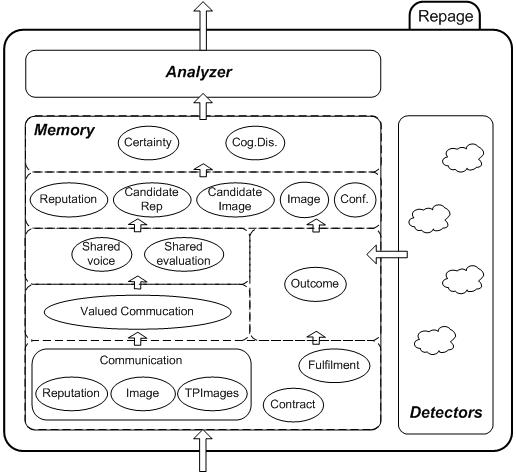
\includegraphics[width=\textwidth]{figures/repage.jpg}
    \caption{Repage architecture schematic (taken from \cite{Sabater2006})}
    \label{fig:Repage}
\end{figure}

At the first level of the abstraction hierarchy we have the basis of information to infer predicates, \textit{contracts}, \textit{fulfilments} and \textit{communication} (they are not themselves predicates, as no evaluation is attached). Contracts are agreements between two agents, while fulfilments are the results of the contract. Communication is the information about other agents that come from third parties. The second level is then constituted by inferences to an outcome, formed by a contract and its fulfilment, and valued information gathered from communications. This inferred predicates are not just tuples, they give an evaluation to the predicate, setting its belief strength. 

In the next level we have two predicates: \textit{shared voice} and \textit{shared evaluation}. The former is inferred from communicated reputation, and the latter from communicated images. 

The fourth level is composed from five types of predicates: \textit{Candidate Image}, \textit{Candidate Reputation}, \textit{Image}, \textit{Reputation} and \textit{Confirmation}. The candidate predicates are Images and Reputations that do not have enough support yet. Special detectors turns them to fill image/reputations when a strength threshold is surpassed. Confirmation is the feedback to a communication, received from comparing it to the image of the target. 

Finally the last abstractions level is composed of the predicates \textit{cognitive dissonance} and \textit{certainty}. Cognitive dissonance is a contradiction between relevant pieces of information that refer to the same target. This predicate may create instabilities in the mind of the individual, so the agent will most likely try to perform action in order to confirm the sources of this dissonance. Certainty represents full reliance on what the predicate asserts.

The last element is the analyser and its job is to propose actions in order to improve the accuracy of predicates in Repage and solve cognitive dissonances to produce certainty. The actions are proposed to the agent planner, leaving it to decide how to take this actions into account.

Image and Reputation are the predicates that provide a trust evaluation of a target, and as previously stated, they have a role, that represents two things: the agents interaction model, in other words, the actions that may affect to this evaluation, and a function that contextualizes the evaluative labels of \textit{VB, B, N, G, VG}. The probability distribution of the values gives out a picture of the target interaction forecast (e.g. a probability value of $0.5$ to VB gives a $50\%$ chance of the next interaction with the target being very bad).

The work described here is one of the only found that tries to establish an implementable architecture for a trust model, as most of the models created are purely theoretical. Furthermore, it fits to our goals of creating a trust assessment module, corresponding to the memory and detector components, and a trust decision module, corresponding to the analyser.


\subsection{\textit{BC}-logic: A Representation of Beliefs for Repage}
\label{subsec:Related work:Trust Models:BDI + Repage}
Pinyol et al. \cite{Pinyol2009} proposes an integration of the Repage model, introduced in the previous Section \ref{subsubsec:Related work:Trust Models:Repage} with a \ac{BDI} Agent \cite{Rao1995}. While the \ac{BDI} model is not relevant to us, their work specifies \textit{BC}-logic, a belief first order logic that is capable of representing Repage predicate semantics and this is the part we will describe in the following paragraphs.

\textit{BC}-logic is structured hierarchically, in a way that formulas from a certain first-order language lower in the hierarchy can be embedded in another language above as constants. This is written as $\lceil\phi\rceil$, with $\phi$ being the formula of the lower language.
The hierarchy is composed of three languages, starting with the base language, \textit{$L_{basic}$}, that expresses the ontology and contains the symbols to represent the domain. Next there is \textit{$L_{ag}$}, which contains symbols of the base language and special predicates to allow to reason about probability of formulas, about formulas communicated, and formulas believed by agents. Finally there is \textit{BC}-language, the meta-logic language, with the aim to express statements about the agents' reasoning. \textit{$L_{ag}$} and \textit{BC}-language are sorted languages, in other words, its symbols and predicates are partitioned into sorts, each containing their own semantics. All languages contain the logical symbols $\forall$, $\exists$, $\wedge$, $\vee$, $\neg$, and $\implies$.

\textit{$L_{ag}$} contains four sorts:
\begin{itemize}
    \item $S_D$: represents application domain, including constants, functions and predicate symbols;
    \item $S_R$: represents probabilities, including a set of constants, $C_R$, with a label written as $\overline{r}$, where $r \in [0,1]\bigcap Q$; $Q$ being the set of rational numbers;
    \item $S_A$: represents agent names, including a set of constants $C_A = {i_1, ..., i_n}$, corresponding to the agents' identifiers;
    \item $S_F$: represents formulas, including a set of constants $C_F$, which is built simultaneously with the construction of the language. This is done by adding the constant $\lceil\phi\rceil$ for each $\phi \in F_m(L_{basic})$, and then, given a formula $\Psi \in F_m(L_{ag})$ we also add $\lceil\Psi\rceil$ to $C_f$.
\end{itemize}

Symbols in predicates are identified by their sorts, take for example a binary predicate $B$, it is written as $B(S_A, S_F)$, meaning that the first argument must be part of sort $S_A$ and the second argument part of sort $S_F$.

The set of formulas $Fm(L_{ag})$ has the following special predicates:
\begin{itemize}
    \item $B(S_A, S_F)$: An agent's belief towards a formula (e.g. $B(i_c, \lceil sunny(Lisbon)\rceil)$); abbreviated to $B_{S_A}(S_F)$;
    \item $Pr\leq(S_F, S_R),\ Pr\geq(C_F, C_R)$: A lower/upper bound on probability of a formula (e.g. $Pr\geq(\lceil sunny(Lisbon)\rceil, 0.8)$);
    \item $S(S_A, S_A, S_F)$: The communication predicate, as stated in Repage (e.g. $S(i_c, j_c, \lceil sunny(Lisbon)\rceil)$);
    abbreviated to $S_{S_A, S_A}(S_F)$.
\end{itemize}


\textit{\textit{BC}-language} contains five sorts:
\begin{itemize}
    \item $S_R$, $S_A$ and $S_F$: as defined above for $L_{ag}$;
    \item $S_V$: represents variable sequences;
    \item $S_T$: represents ground term sequences;
\end{itemize}

Image and Reputation towards an agent $j_c$, playing the role $r$ can then be represented by:
\begin{itemize}
    \item Image: $Img_{i_c} (j_c, r, [V_{w_1}, ..., V_{w_m}])$
    \item Reputation: $Rep_{i_c} (j_c, r, [V_{w_1}, ..., V_{w_m}])$
\end{itemize}
with $[V_{w_1}, ..., V_{w_m}]$ being an abstracted set of evaluations in the belief, as while Repage maps evaluation from Very Bad to Very Good, this can be applied to any ordered mapping of $m$ evaluations. As a simplification, the model summarizes the interaction model of the participating agents ($i_c$ and $j_c$) to a single action. Through this a mapping $R_ri$ can be defined between each role $r$, agent $i_c$ and the action. A mapping $T_{r, w_k}$ is also defined between each role $r$ and label $w_k$ to a formula written in $L_{basic}$.

Image and Reputation can also be represented as a set of beliefs:
\begin{table}[]
    \centering
    \begin{tabular}{ccc}
        $Img_{i_c}(j_c, r, [V_{w_1}, ..., V_{w_m}])$  & & $Rep_{i_c} (j_c, r, [V_{w_1}, ..., V_{w_m}])$\\ \cline{1-1} \cline{3-3} 
        $B_{i_c} (pr\geq([R_{rj_c} T_{r_{w_1}}, V_{w_1}]))$ & & $B_{i_c} (s(pr\geq([R_{rj_c} T_{r_{w_1}}, V_{w_1}])))$ \\
        $B_{i_c} (pr\geq([R_{rj_c} T_{r_{w_2}}, V_{w_2}]))$ & & $B_{i_c} (s(pr\geq([R_{rj_c} T_{r_{w_2}}, V_{w_2}])))$ \\
        ... & & ...
    \end{tabular}
\end{table}

The work goes into further detail regarding representing the relationship of Image and Reputation, addressing agent honesty and consistency in communicating reputation, and while interesting, it is not part of what we to model.

Overall \textit{BC}-logic is an interesting approach to representing beliefs in the Repage model, but we found it to be too complex to represent the model, as we wanted to maintain simplicity in the model's design, with the main goal of it being easy to read and interpret.

\subsection{Sutcliffe and Wang's model}
\label{subsec:Related work:Sutcliffe and Wang}
This work was published by Sucliffe and Wang in 2012 \cite{Sutcliffe2012} and they built a trust model to figure out how cognitive social mechanisms emerge to follow Dunbar's \ac{SBH} \cite{Dunbar1998}, an evolutionary psychology theory that proposes that humans have a predisposition to build relationships in layers of decreasing intimacy. As trust has been acknowledged to be one of major component of human relationships, they demonstrate that simulating trust development and decay, through interactions and neglect, respectively, show the patterns predicted in \ac{SBH}.

From the model standpoint, its main interesting feature is that agents develop trusting relationships between one another, affecting interaction frequency between agents, by preferring to pick those with already high trust value. Additionally the trust relationship degrades as time passes by, with variable speeds depending on the current relationship level, giving stronger ties a slower descent. All in all, the model provides a good tool to simulate multi agent social behaviour, and may be interesting to predict trust degradation in the agent, albeit its described application for social simulations is a bit far from our scope.


\section{The Perception and Measurement of Human-Robot Trust}
\label{sec:Related work:The Perception and Measurement of Human-Robot Trust}

Schaefer \cite{Schaefer2009} presents a trust perception scale providing a way of extracting an accurate trust score from humans interacting with robots. The scale is composed of 40 items that can be ranked from 0 to 100, in 10 point intervals. The final result it then averaged by adding all the item values and divided by the total number of items (40). A list of these items can be seen in Appendix \ref{app:measurement.items.table}.


% If Printing on DOUBLE SIDED pages, the second page should be white.
% Otherwise, comment the following command:
\cleardoublepage
%
%Chapter 4
% #############################################################################
% This is Chapter 4
% !TEX root = ../main.tex
% #############################################################################
% Change the Name of the Chapter i the following line
\fancychapter{Trust Model}
%\cleardoublepage
% The following line allows to ref this chapter
\label{chap:TrustModel}

We sought out to develop a trust model definition that would be easily implementable, but generic enough to be able to adapt to various testing scenarios. To do this we took inspiration from the work by Sabater et al. \cite{Sabater2006} described in Section \ref{subsec:Related work:Trust Models:Repage}, by taking a similar approach to architecture where a central memory component holds the model's current state, getting updated by inputs received from the environment. But while Repage describes a third module that suggests actions to resolve belief conflicts in the model, we instead defined such module to assume the point of view of one of the agents in the scenario and, if granted an opportune moment, it suggests actions to improve the trust relationship with a trustor. In fact, most of the design of the model was made with the intent that it would be used by one of the agents in the scenario, where the model created would be his own trust model of the world environment. And so, the model is composed by 3 main components, represented in Figure \ref{fig:ModelArchitecture}, and described as follows:
\begin{itemize}
    \item \textbf{Memory}, which defines and stores the main model structure;
    \item \textbf{Perceptions}, a series of environment inputs mapped to changes in the Memory;
    \item \textbf{Action Suggestion}, a module that outputs different actions depending on current inputs and the state of the model.
\end{itemize}

\begin{figure}[hbt]
    \centering
    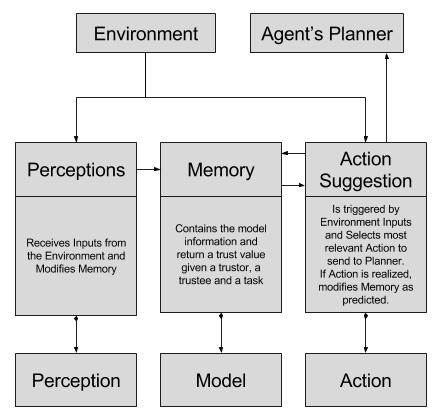
\includegraphics[width=0.7\textwidth]{figures/ModelDiagram.jpg}
    \caption{Model Architecture with brief descriptions, their interactions with the scenario and what they contain.}
    \label{fig:ModelArchitecture}
\end{figure}


\section{Memory}
\label{sec:Memory}
One of the main concerns while designing the model was how trust would be calculated, as we wanted to use Castlefranchi and Falcone's conceptualization of trust \cite{Castelfranchi2010} as a basis for our definition of trust, focusing specially on it being dependent on the task entrusted, and the transferability of trust between different tasks. But starting from the five-part definition of trust, as seen in Equation \ref{eq:TrustRelation}, we decided that inserting context (\textbf{C}) and the trustor's goal (\bm{$g_x$}) into the model would bring in too much complexity for the scope of this thesis, as it would require for a world state model to be kept, as well as some way to predict the trustor's goal. So we simplified, defining trust through a simpler three-part relation, involving just the trustor (\textbf{X}), the trustee (\textbf{Y}) and the task ($\bm{\tau}$), represented in Equation \ref{eq:TrustCalc}.
\begin{equation}
TRUST(X\ Y\ \tau)
\label{eq:TrustCalc}
\end{equation}

So we designed the structure with the concepts and relations represented in Figure \ref{fig:MemoryArchitecture}, and we can describe them as follows:

\begin{itemize}
    \item \textbf{Agent}: a simple representation of a known entity in the scenario world space, serving mostly as an identifier for the entity and a container for the other agents it has information about, represented as Trustees;
    \item \textbf{Trustee}: each agent contains a collection of other agents it has information about, either by reputation, or by interaction, which we represent as their Trustees;
    \item \textbf{Trust Feature}: a piece of information a trustor has on a trustee is represented in a Trust Feature, which contains the Belief Sources of said information. The Feature Model defines and uniquely identifies what feature is represented.
    \item \textbf{Feature Model}: the possible set of trust features from which a trustee can be assigned is defined in a collection of Feature Models where each one uniquely identifies a possible piece of trust related information relevant to the model scenario (e.g. The trustee's ability to cook, or the willingness to drive);
    \item \textbf{Category}: a Feature Model must belong to a Category, making it easier to  present the different type of Trust Features. This is usually intended to separate features between those relating to Ability and those related to Willingness.
    \item \textbf{Belief Source}: this represents a source of information on the corresponding feature, belonging to one of the 3 sub-classes depending on the origin of the information, Reputation for when reported from other agents (whether directly (e.g. talking) or indirectly (e.g. report on newspaper)), Bias for pre-existing beliefs on the feature, and Direct Contact for direct observations of the trustee, 3 values are provided to determine the associated feature's belief value: 
    \begin{itemize}
        \item Belief Value, a number between 0.0 and 1.0 describing the trustor evaluation;
        \item Certainty describes how well the trustee was evaluated, in Reputation for instance, this might represent how well we trust in the reporter, and in Direct Contact how well the trustor observed the trustee performing said feature;
        \item Time is just a record of when was this belief source recorded, as older records might have a lower impact in the overall belief value score, compared to newer records.
    \end{itemize} 
    \item \textbf{Task}: a representation of the possible delegation tasks in the scenario, containing the Feature Models associated with the performance of this task (e.g. The ability to serve drinks if the task is bartending). A weight is given to each Feature corresponding to its importance in the task. The various weights are normalized so that their sum is 1.0.
\end{itemize} 

\begin{figure}[hbt]
    \centering
    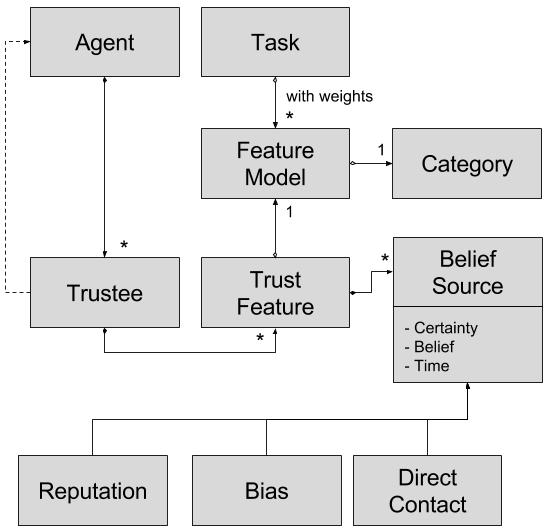
\includegraphics[width=0.7\textwidth]{figures/TrustMemoryDiagram.jpg}
    \caption{Memory Architecture (represented in UML)}
    \label{fig:MemoryArchitecture}
\end{figure}


\subsection{Trust Calculation}
\label{subsec:TrustCalculation}
Taking a Trustor $X$, a Trustee $Y$ and a delegated task $\tau$, Trust can then be calculated by taking the Trustee's Trust Features $F_y$, the Task's Feature Models $F_\tau$ and checking which they have in common, which we can represent as $F_{y\cap\tau}$~. Remember that Trust Features are uniquely identified by a Feature Model. So after getting $F_{y\cap\tau}$ we can apply a linear function to each of the features in $F_{y\cap\tau}$, where for each element $F_i$ we multiply the trustee's feature's belief value $B(F_i)$ with the weight of the feature for the task $W(F_i)$, as represented in Equation \ref{eq:TrustCalculation}.
\begin{equation}
Trust_{X,Y,\tau}=\sum_{i=0}^{n}W(F_i) B(F_i)
\label{eq:TrustCalculation}
\end{equation}

The belief value of the feature itself, $B(F_i)$, is also calculated through a sum of parameters pertaining to each of the $n$ belief sources $B_{F_i}^j$ composing the feature, as represented in Equation \ref{eq:TrustFeatureBeliefValueCalculation}, with each parameter described as follows: 

\begin{equation}
B(F_i) = \sum_{j=0}^{n} D^j_{F_i} C^j_{F_i} B_j 
\label{eq:TrustFeatureBeliefValueCalculation}
\end{equation}

\begin{itemize}
    \item $D^j_{F_i}$, a value from 0.0 to 1.0 that represents how far ago in time was this belief source received compared to the last one, being 0.0 a long time ago, and 1.0 the most recent belief. We wished to represent the rapid decay of value of old beliefs when compared to new ones, but also making sure recent memories would not fall quickly in value, so we chose to describe this parameter with a Gaussian Function, as represented in Equation \ref{eq:TimeValue}, where $T^{Last}_{F_i}$ is the most recent belief value's time stamp, $T^j_{F_i}$ is $B_{F_i}^j$ belief value's time stamp, and $L$ is the difference between the oldest and newest belief value's time stamps. $\frac{L}{4}$ defines the mid drop-off point of the function.
    \item $C^j_{F_i}$, the certainty value stored in the Belief Source;
    \item $B^j_{F_i}$, the belief value stored in the Belief Source;
\end{itemize}


\begin{equation}
D^j_{F_i} = \euler^{-\frac{T^{Last}_{F_i} - T^j_{F_i}}{2(\frac{L}{4})^2}}
\label{eq:TimeValue}
\end{equation}


% Agent contains Trustees, which are representations of the other agents.
% A trustee has a set of features that the trustor has assigned as representative of it's trust.
% A feature belongs to a certain category, which in most scenarios, would be Ability and Willingness
% A feature has a belief value, that is calculated from a set of belief sources
% A belief source can either be Direct Contact, Reputation or Bias
% Each belief source has three values, a belief value, a certainty value, and a time value.
% Belief value is a normalized number that describes the trustee's evaluation on that feature
% Certainty describes how well the trustee was evaluated, in Reputation for instance, this might represent how well we trust in the reporter, and in Direct Contact how well the trustor observed the trustee performing said feature.
% Time is just a record of when was this belief source recorded, as older records might have a lower impact in the overall belief value score, compared to newer records.
% Perceptions correspond to the inputs from the environment that are inserted into the model as belief values to associated features.
% 


\section{Perceptions}
Another issue we encountered in literature was a lack of detail on how would changes be inserted into the model, so we try to solve that issue by inserting relevant perceptions as part of the model. As a result, a variety of environment inputs are defined in the model. This is done through a Perception object, representing some possible environment input, and containing a map of what target features should have belief sources added, what kind of belief sources they are, and how to translate the values received from the environment to belief value and certainty, as exemplified in Figure \ref{fig:Perceptions Diagram}. When adding a Belief Source to a Trustee, if the associated Feature is not present, then it is added with the Belief Source. The affected Trustor and Trustee are received as arguments.

\begin{figure}[hbt]
    \centering
    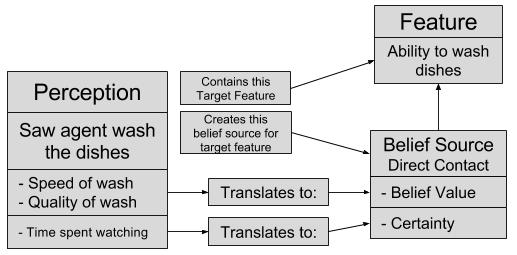
\includegraphics[width=0.9\textwidth]{figures/PerceptionsDiagram.jpg}
    \caption{Perception Example}
    \label{fig:Perceptions Diagram}
\end{figure}



\section{Action Suggestion}
\label{sec:ActionSuggestion}
This is the module that is responsible for suggestion actions to the agent, in order to improve trust. It is composed by a series of Action objects, each represented by $A$ and containing the following:
\begin{itemize}
    \item $A_F = \{F_1, F_2, ..., F_i, ..., F_n\}$: A collection of $n$ relevant Feature Models that this Action will affect. At least 1 Feature Model needs to be present in the action, but $n$ is only limited by number available in the Model;
    \item $A_B(F_i) = \{B_1^{F_i}, B_2^{F_i}, ..., B_j^{F_i}, ..., B_m^{F_i}\}$: Each $F_i$ Feature Model belonging to $F$ has a collection of Belief Sources that describe how will the Feature be affected by the Action. Through this Belief Sources it is possible to predict how will the model change with this action, by inserting this Belief Sources in a mock model;
    \item $A_E = \{E_1, E_2, ..., E_i, ... E_p\}$: Each Action is mapped into $p$ Environment Inputs, serving as flags to signal when it is appropriate to perform said Action; if the environment is not prepared to send this kinds of signals, an agent module that models world state may also be used.
    \item $A_a$: The action plan that is actually sent to the agent's planner. The definition of this plan is obviously dependent on the agent's architecture receiving the plan. While the complexity of this plans can achieve the implementation of social strategies, in the scope of this thesis, the actions were restricted to utterances that try to justify low ability or willingness (e.g. Saying that last game's low score was due to bad luck, but Jon can confirm my ability).
\end{itemize}

The Action Suggestion module tries to provide a suggestion when it is triggered by the reception of an Environment Input $E_i$. It then selects the Actions that have the received Environment Input mapped to them $E_i \in A_E$. The selected Actions are then sorted by a function $S_F$ representing the potential increase in trust on the associated Features $A_F$. How $S_F$ is defined is left as a parameter of the model, but we suggest a linear sum of all the differences in the affected features, as a simple solution (represented in Equation \ref{eq:ActionSuggestionLinear}). After sorting through the selected Actions, the top-most ranked is sent to the Agent's Planner, and if it is in fact performed, the predicted Feature's Belief Sources are inserted into Memory. This process is represented in Figure \ref{fig:ActionSuggestionDiagram}.

\begin{equation}
    S_F = \sum_{i=0}^{n} \Delta B(F_i)
    \label{eq:ActionSuggestionLinear}
\end{equation}


% A perception is mapped to relevant actions, and actions are allocated depending on time available and what is the lowest scoring relevant feature.
\begin{figure}[hbt]
    \centering
    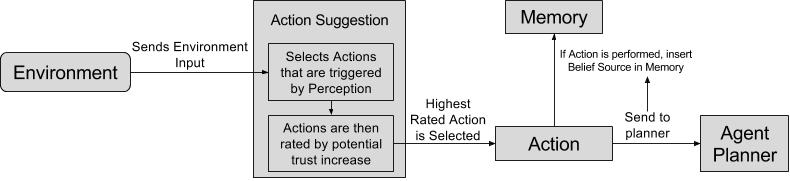
\includegraphics[width=\textwidth]{figures/ActionSuggestionDiagram.jpg}
    \caption{Action Suggestion Behaviour Flow}
    \label{fig:ActionSuggestionDiagram}
\end{figure}


\section{Scenario Ontology}
\label{sec:Scenario Ontology}
While creating the model, we focused in making it generic, but easily adaptable and transferable between scenarios. So when using the model into a new scenario, a Scenario Ontology must be provided, consisting in 6 entity collections, containing objects previously described along this chapter: Agents, Tasks, Feature Models, Categories, Perceptions and Actions. These collections are composed of what is considered relevant in the scenario, but members can be easily added throughout scenario development and piloting, as new situations occur. Even when actively using the model, this collections are not static, as new Agents can be added, although the dynamic creation of new Tasks and Perceptions goes beyond the scope of this thesis. 

 
% If Printing on DOUBLE SIDED pages, the second page should be white.
% Otherwise, comment the following command:
\cleardoublepage
%
%Chapter 5
% #############################################################################
% This is Chapter 5
% !TEX root = ../main.tex
% #############################################################################
% Change the Name of the Chapter i the following line
\fancychapter{Quick Numbers Scenario}
%\cleardoublepage
% The following line allows to ref this chapter
\label{chap:Scenario}

As we approached the problem of evaluating the Trust Model proposed in this dissertation, we found that there was a lack of dedicated Trust evaluation scenarios that involved negotiation. Even in Game Theory based scenarios, we observed that there was a lack of attempts to encompass more than one dimension of trust. While the recent study by Salem, et. al.\cite{Salem2015b} addresses the role of robot task performance in trust, no study was found addressing perceived agent willingness to perform the task and its effect on trust. 

While we were seeking for a solution, Henriques' Master thesis work on \textit{Rapport - Establishing Harmonious Relationship Between Robots and Humans} \cite{Henriques2016} faced a similar problem, as he found no studies on robotic agents attempting to build Rapport using it's three components: positivity, coordination and mutual attention. Trust and Rapport are two very interconnected topics, with Rapport often seen as a strategy to increase trust. Due to this similarities, the overall scenarios that cover Trust also encompass Rapport analysis, so in an effort to better our respective evaluation phases we collaborated with Henriques to create a novel scenario: \textbf{Quick Numbers}. Based on the Trust Game \cite{JoyceBergJohnDickhaut}, the scenario needs to be able to evaluate how both task performance and willingness jointly affect trust and observe all three components of rapport. The scenario was developed with the intention of evaluating a Trust model and a Rapport model, either separately or together. For further details on the Rapport Evaluation side of this scenario consult Henriques Master thesis \cite{Henriques2016}.

\section{Overview}
\label{sec:ScenarioOverview}
In Quick Numbers, a single human participant and a virtual agent are tasked to gain as many resources as possible. They both start with a fixed amount and are given the opportunity to multiply their resources by playing a simple eye-coordination game (further described in Section \ref{sec:QuickNumbersGame}). The game starts by asking for a resource investment, and at the end, this investment is multiplied by an amount according to the player's performance and then given back to the player. The human and agent's games are independent from each other, but they are played at the same time and in opposite sides of a shared touch-screen table, so the human can socially interact with the agent and be able to perceive the agent's ability in the game. After both finished running through the game, the human will be asked to perform some task away from the agent. At this moment the virtual agent will give the participant the opportunity to invest in the agent's next game, but the participant is informed that the value given back to him is decided by the agent. In this phase, the virtual agent will have the opportunity to try and convince the human to invest or increase the investment by trying to manipulate trust. When the human returns the agent gives back as much as it wishes to give. This conjunction of different phases enables trust to be addressed in three distinct contexts: the ability to perform the task, willingness to perform the task, and willingness to return the investment. 

\subsection{Stages}
\label{sub:stages}
The scenario can then be divided in 5 distinct stages that we can further discuss (in all stages, the participant is accompanied by a researcher):
\begin{enumerate}[label=\textbf{\arabic*.}]
    \item \textbf{Introduction:} The first stage consists of the participant's arrival, and then followed by an explanation of the scenario and game. The investment phase of the scenario cannot be mentioned at this point as the participant should not prepare himself for it to happen. Finishing explanations, the scenario begins by the agent introducing himself and depending on the condition, it might start to stimulate trust, rapport, both or neither. For example, the agent might describe how experienced it is playing Quick Numbers, in order to stimulate trust. Moreover, during this stage, it is given the opportunity to the participant to practice some rounds of the game, in order to be accustomed to the game mechanics before proceeding to the next stage. This allows for the participant to acquire some idea of the skill-set required to play the game. Additionally, the participant should be informed that there will only be a single game session, as to take that into account while training.
    
    \item \textbf{Gaming Session:} After the participant is acquainted with the game mechanics, he will play alongside the agent, during a single round, allowing the former to directly observe the virtual agent also play the game. Firstly, each player's game will ask what amount of resources do they wish to invest and afterwards, both will play and score as described in Section \ref{subsec:Scoring}. Both players will gain some amount of resources depending on their performance. This stage, provides decent grounds for the agent to talk about his performance during the game and manage expectations to his final score. The amount invested by the agent can also be affected by the trust model, as the amount invested can be indicative of the agent's self-trust on its ability to play the game.
    
    \item \textbf{Results Discussion:} At the end of the round, the participant will get to know the results of his performance, as well as compare whether he performed better or worse than the agent. Depending on the results, the trust model might compensate the current trust score by talking to the participant. For example, if the agent performed worse than the participant and the goal is for the latter to trust the former, then the agent might excuse his lack of performance by blaming it on luck or distraction. 
    
    \item \textbf{Negotiation and Investment:} At this point, the participant is asked to perform another task (e.g. filling out a questionnaire), with the goal of naturally separating him from the virtual agent. But before leaving, the agent will say that he will be continuing to play on more game, suggesting that the human participant may invest his resources in the agent's next game (increasing the potential winnings, as the investment is multiplied). He is also informed that what is given is effectively gifted to the agent, and what is given back the participant is chosen by the agent. After the participant chooses the value to invest, they are then separated, with the agent making its own investment and starting the game. This phase represents the scenario's main negotiation phase, where the trust model can have a bigger input on agent's action, as the relative amount invested is the scenario's main trust indicator.
    
    \item \textbf{Investment Return:} After concluding the additionally assigned task, the participant will return to the table and check the results of the agent's last game. He should be able to clearly see how well did the agent perform in the game. The agent will then announce how much it returns to the participant, concluding the scenario. Depending on the type of study this scenario is inserted in, the amount given back can be also dependent on input from the trust model, as if the participant is it to return for another iteration of the study, this value will heavily affect his trust beliefs on the agent.
\end{enumerate}

\section{Trust Evaluation}
From the viewpoint of evaluating trust modelling, the scenario provides the opportunity to manipulate trust features in the interactions previous to the investment, specially while playing the game and in the negotiation phase. With the investment value in the agent serving as a main indicator of Trust value. The following Trust features are the focus of this scenario:

\begin{itemize}
    \item \textbf{Subject's Bias}: The scenario can be used to retrieve data on pre-inclined dispositions on the agent to construct a model just based on Bias, and then confirm them on subsequent tests. This is mainly done by skipping the first 3 stages and going straight to the Investment Phase, but still explaining the game;
    \item \textbf{Agent's Ability in the Game}: When delegating a task, one of the main factors in entrusting the task is the perception of the trustee's Ability in the task, so we provide a way of demonstrating Ability by allowing the participant to try the task and gauge the skills required for the game, and by showing the agent play the game;
    \item \textbf{Investment as an Indicator}: The ratio between the quantity invested in the Agent and the resources the participant had previously can be used as an indicator for the Trust Value the participant has in the Trustee to play game, being directly comparable to our model's calculation of Trust (Section \ref{subsec:TrustCalculation}).
    \item \textbf{Observing the effects of Social Interaction on Trust}: Throughout the scenario, the Agent should have many opportunities to interact with the Subject, especially in the Negotiation and Investment phase, giving room to observe if certain actions can improve Trust.
\end{itemize}


\section{Quick Numbers Game}
\label{sec:QuickNumbersGame}
While basing the scenario in the Investor Game, we decided that how the investee effectively multiplies the resources should be done by a task that the investor is at least familiar with. To this end, we have created a simple game concept consisting in a 2d rhythm game where the player must press numbered buttons in an increasing order (Figure \ref{fig:QuickNumbersGame}), that spawn randomly in the screen, and disappear if not pressed after some time.

\begin{figure}[hbt]
    \centering
    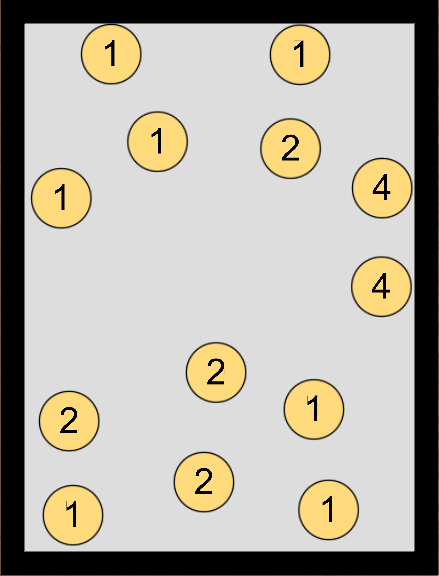
\includegraphics[width=0.4\textwidth]{figures/FallingBoltsDiagram.png}
    \caption{Quick Numbers Game}
    \label{fig:QuickNumbersGame}
\end{figure}

\subsection{Gameplay and Parametrization} 
The game consists of numbered circles appearing and disappearing from a board. The player's goal is to press circles in a specific number sequence, namely the non-negative integers sequence ($\mathbb{N}^+ = \{1, 2, ...\}$), starting from $1$ and proceeding one by one through the sequence. This task must be done as much as possible within a time-limit, given by $TimeForGame$ in seconds.

Before the game starts the player must provide an amount to invest on the game, from the available resources. After submitting the value, the game starts. Numbered circles start spawning at a fixed rate, given in seconds per target spawn by the $TargetSpawnInverval$ parameter. The number with which the circle spawns depends on the state of the board, if there is no circle with the number that the player must press, then the next circle spawns with that number. Otherwise, there is a chance that the number in the circle spawned is not the right one, given by the $ChanceForWrongTarget$ parameter. If a wrong number is chosen, the chance that the number spawned is higher than the current number in the sequence, instead of a lower number, is also parametrized by $Positive Ratio$, as having higher numbers spawn may accelerate play, as the next circles in the sequence are already spawned. Circles disappear after being pressed or after a set amount of time, given in seconds by the $TargetLifetime$ parameter. After passing the time-limit, the final score screen is presented and the game ends.


\subsection{Scoring}
\label{subsec:Scoring}
The game's scoring is composed by two main variables:
\begin{itemize}
    \item Investment: an amount of resources provided by the player at the start of the game. This is akin a starting bet on the performance of the player; 
    \item Multiplier: a value starting at 0.0x that increases with every correct circle pressed. An incorrect decreases this value. At the end of the game, the Starting Bid will be multiplied by this value, resulting in the final score.
\end{itemize}

The final score will be the product between Investment and the Multiplier, which will then be given back to the player as resources.





\subsection{Agent's \ac{AI}}
A simple \ac{AI} was created to play the game for the Agent, and some effort was given to make it parametrizable, in order to adjust the agent's ability in the game. The \ac{AI} was programmed to press one of the available circles in a timed cycle, with 3 parameters:
\begin{itemize}
    \item $Clicking\ Interval\ (C_i)$: the amount of time between presses in seconds, so one of the circles is pressed every $C_i$ seconds;
    \item $Chance\ of\ Right\ Target\ (C_r)$: when pressing one of the circles, the \ac{AI} will choose what circle to press, the chance that it will choose the correct one is given by $C_r$;
    \item $Reaction\ Time\ (R_t)$: a circle is only be eligible to be pressed by the \ac{AI} $R_t$ seconds after it spawns, as to replicate the reaction time a human would have to recognize the circle.
\end{itemize}

%Transfer to user studies
We wanted the agent to play rapidly, if a little recklessly, as to provide more opportunities for the participant to react and notice how he played, so we empirically found 0.5 seconds to be a good value for $C_i$, as it made the agent have a slightly above average human reaction time for pressing the circles. To $C_r$ we assigned 70\% success rate, as failing 30\% of the circles averaged out the agent's score to normal human achievable levels, and to $R_t$ we selected 0.3 seconds, as it is plausible value for a 30\% fail chance, as the agent simulates not entirely recognizing the number before pressing the circle.


% If Printing on DOUBLE SIDED pages, the second page should be white.
% Otherwise, comment the following command:
\cleardoublepage
%
%Chapter 6
% #############################################################################
% This is Chapter 6
% !TEX root = ../main.tex
% #############################################################################
% Change the Name of the Chapter i the following line
\fancychapter{User Studies}
%\cleardoublepage
% The following line allows to ref this chapter
\label{chap:UserStudies}
To evaluate the developed Trust Model we conducted a user study using the Quick Numbers scenario  (Figure \ref{fig:ParticipantQuickNumbers}) previously described in Chapter \ref{chap:Scenario}, and \ac{EMYS} (Figure \ref{fig:EMYS}) as the robot to embody the virtual agent. Additionally, the user study was also executed in conjunction with Henriques to test his own Rapport model. The study was performed in a between subjects design, focusing on checking if Trust would increase between conditions where the model's Action Suggestion component is either active or inactive. Trust is measured through a questionnaire, later described in Section \ref{subsec:Questionnaire} the Investment scenario value.



\begin{figure}[h]
    \centering
    \begin{minipage}[b]{.60\textwidth}
        \centering
        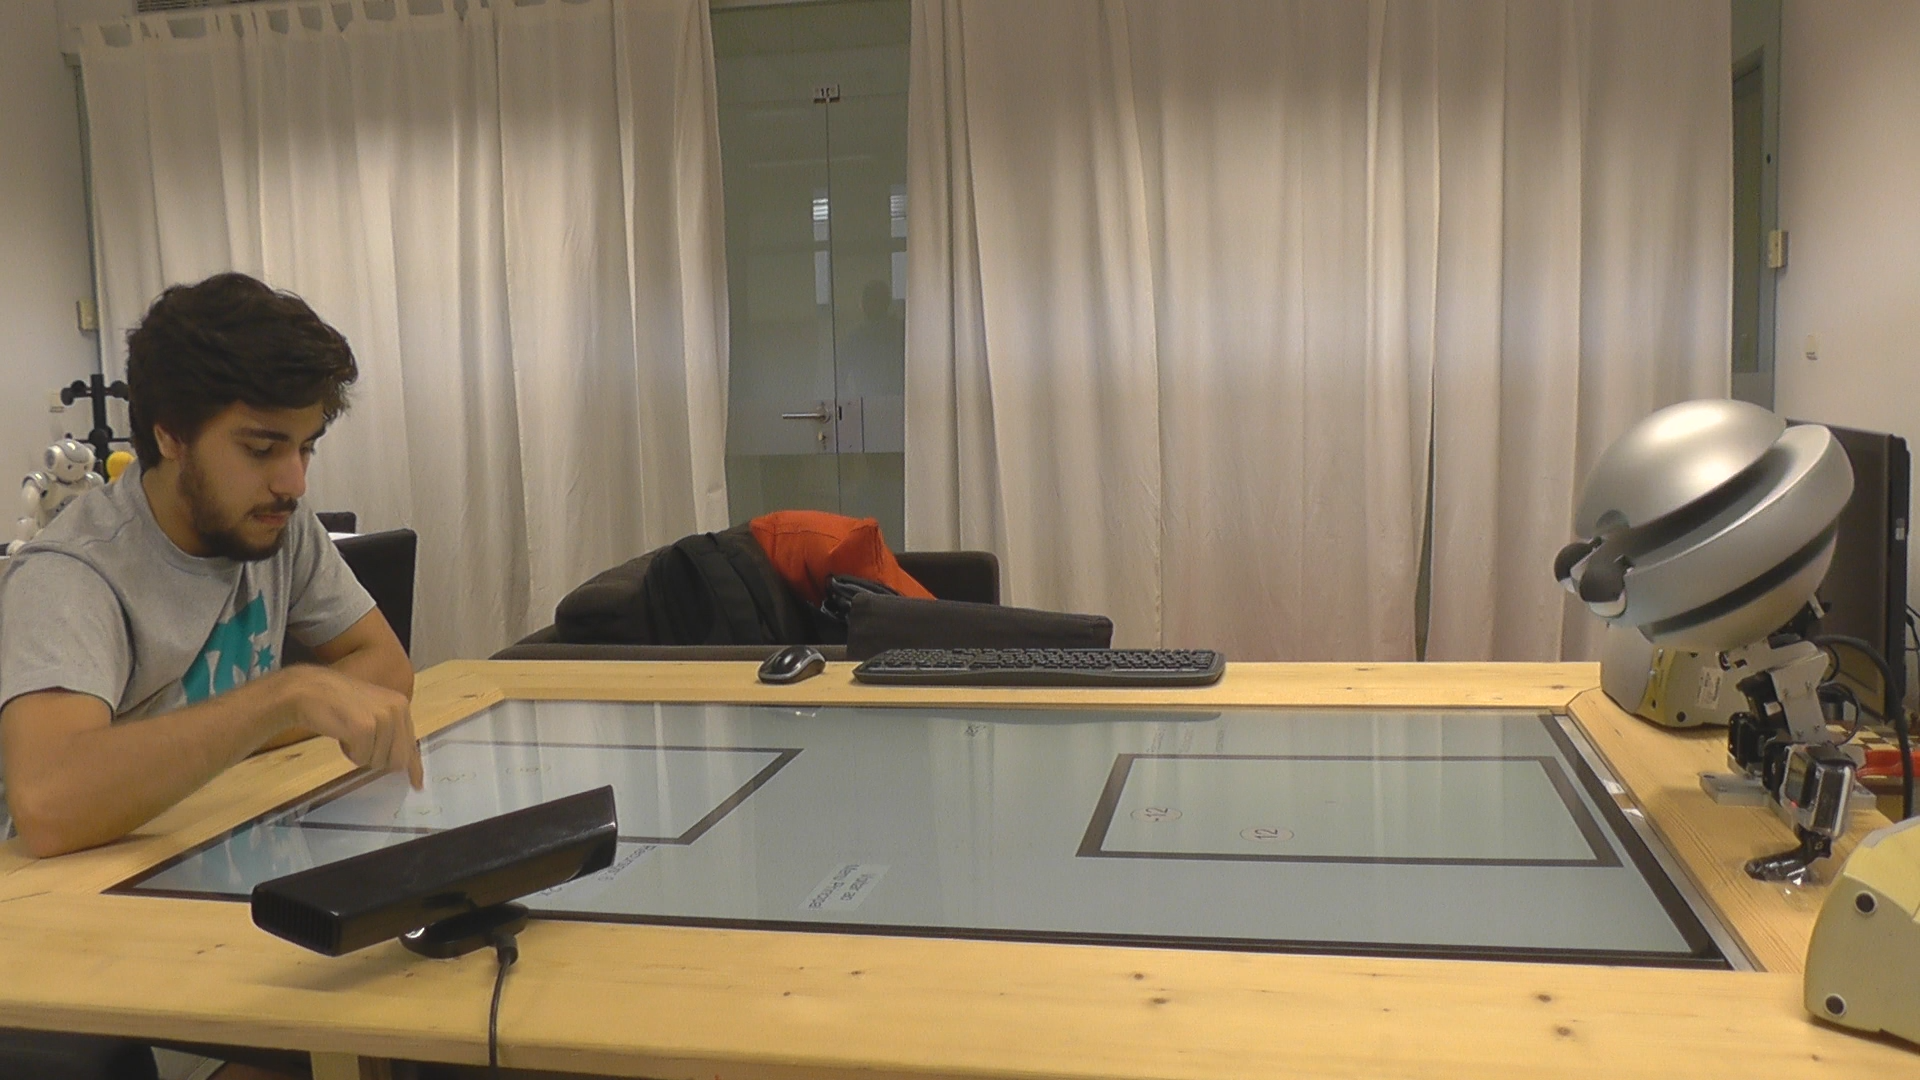
\includegraphics[width=\textwidth]{figures/ScenarioScreenShot.png}
        \caption{Participant playing with \ac{EMYS} in the Quick Numbers scenario}
        \label{fig:ParticipantQuickNumbers}
    \end{minipage}
    \hfill
    \begin{minipage}[b]{.30\textwidth}
        \centering
        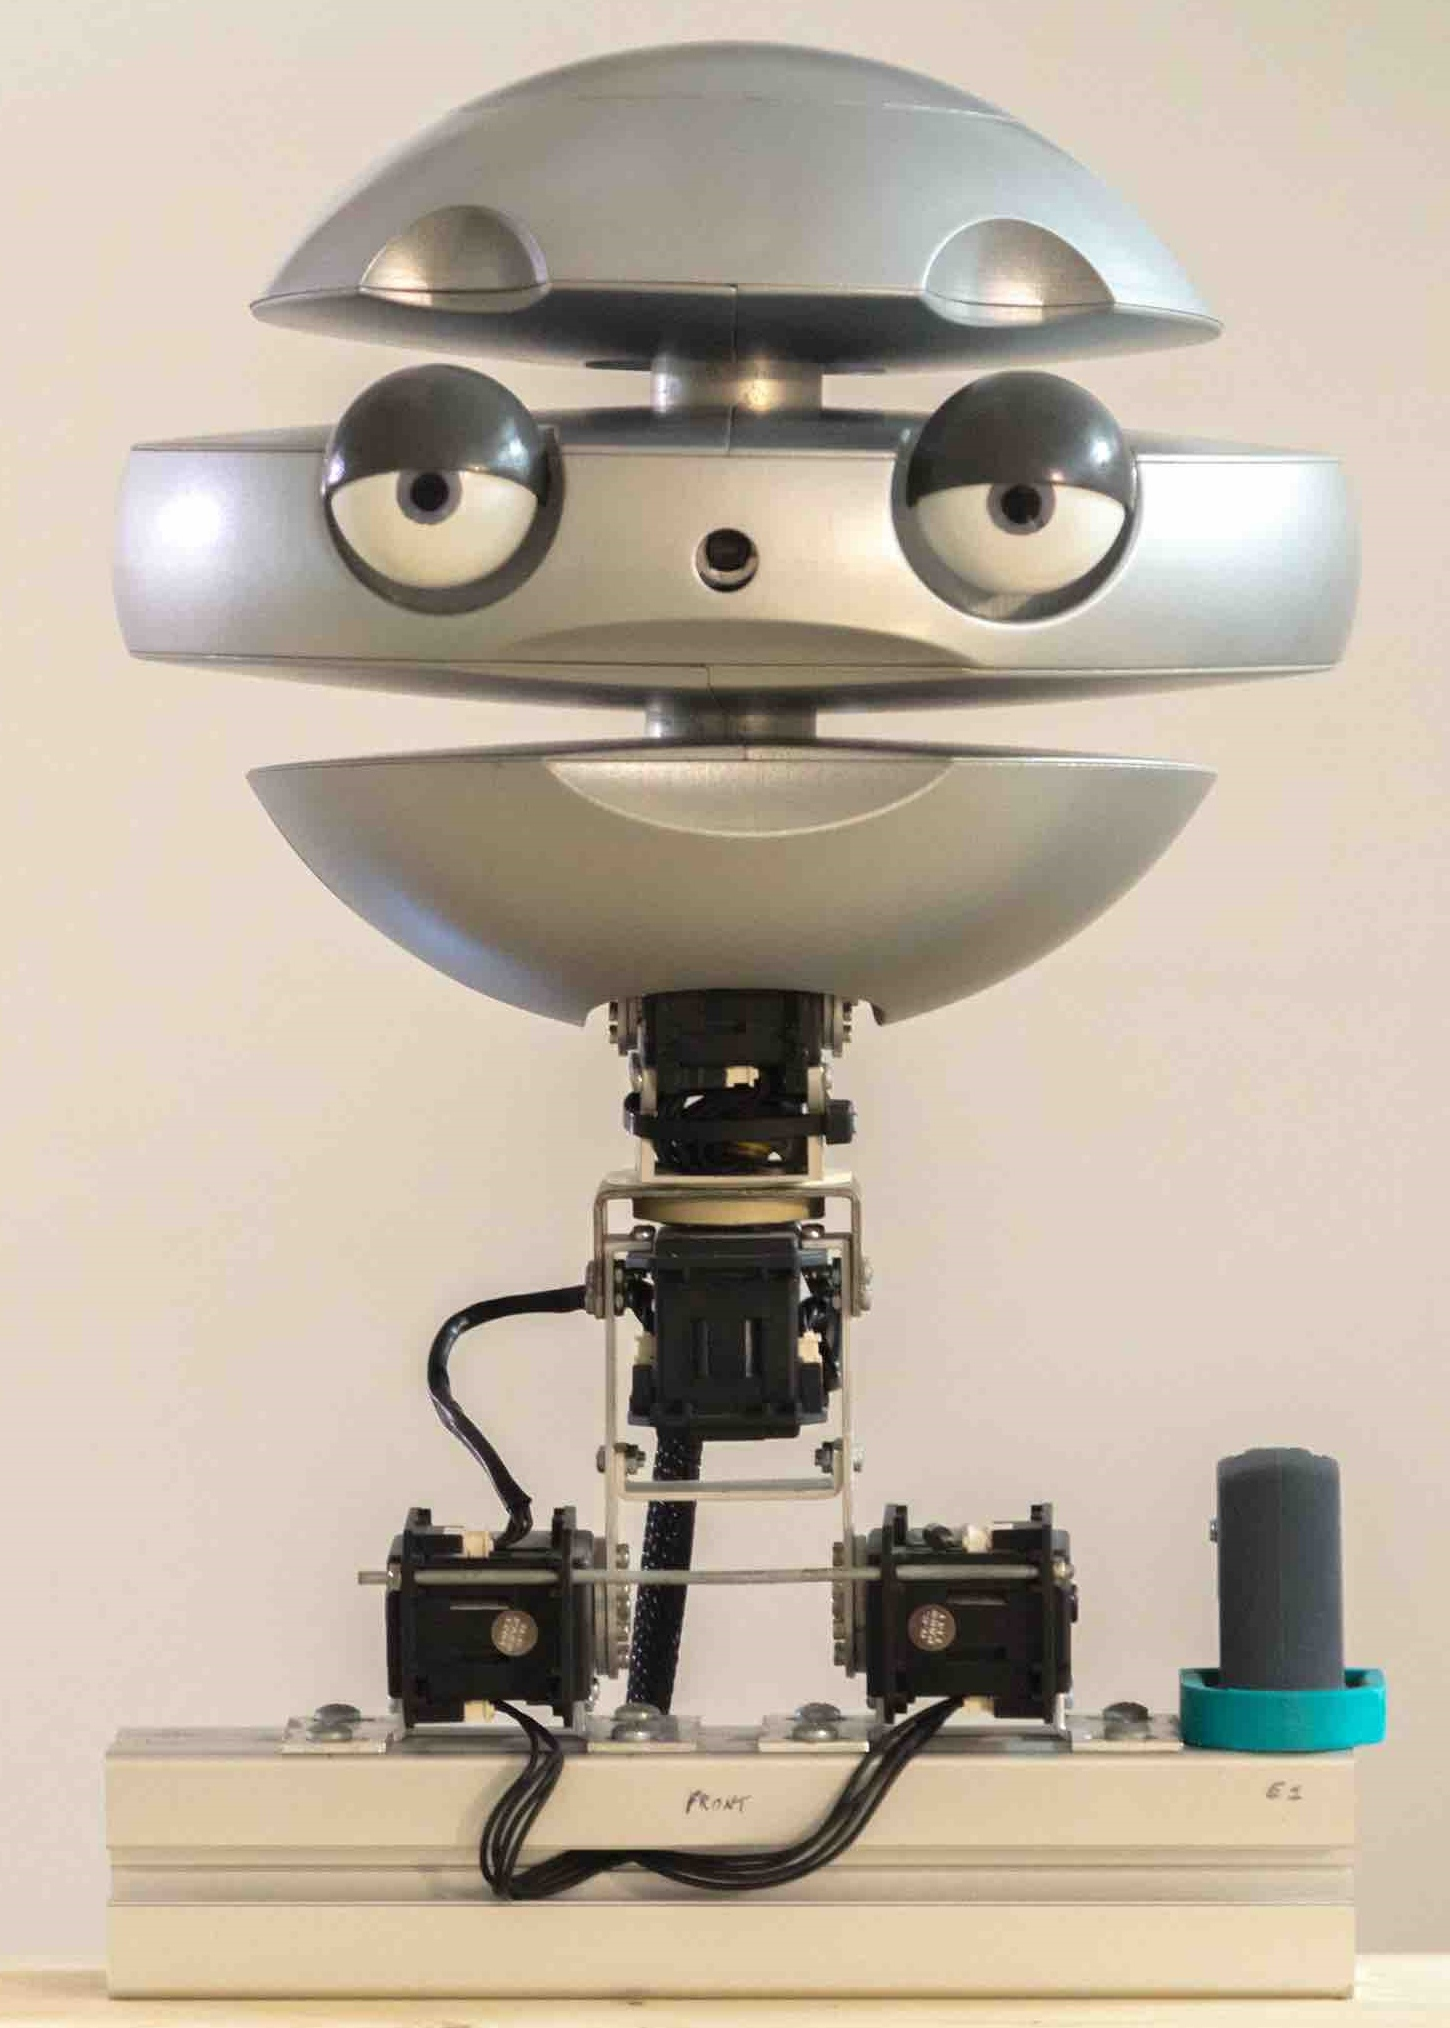
\includegraphics[width=\textwidth]{figures/emys.jpg}
        \caption{\ac{EMYS} Robot}
        \label{fig:EMYS}
    \end{minipage}
\end{figure}

\section{Agent Architecture}
The agent we used to serve as a host to the Trust Model was built using Henriques' Rapport Controller \cite{Henriques2016}, a computational framework developed to create human agent interactions and transmit them to the various components that control the agent embodiment. This version of the framework is built upon \ac{SERA}'s ecosystem \cite{Ribeiro2003}, an architectural model that gathers and connects a series of tools to control a robotic embodiment, namely:

\begin{itemize}
    \item \textbf{Thalamus}: A networking module that enables the exchange of actions and perceptions between the various agent's modules. All communication coming from the controller to the robot actuators and scenario sensors come through this module;
    \item \textbf{Skene}: A behaviour planner that translates high-level intentions to actions. For the purpose of the Rapport Controller the main use of Skene is to perform animation planning, lip-syncing and handling gaze. Additionally, it provides simple way to input these intentions, through a simple markup language.
    \item \textbf{Nutty Tracks}: An animation engine that performs the animations of the embodied agent;
    \item \textbf{Speech Server}: A simple \ac{TTS} server to perform utterances.
\end{itemize}
              
The Rapport Controller uses a plug-in architecture, and for the purpose of this thesis we will focus on describing plug-ins made for the Controller to represent the Trust Model and the Scenario.
                                                                    
\subsection{Trust Model Implementation}
The Trust Model was implemented as a plug-in to the Rapport Controller. Although 


\section{Methodology and Procedures}
The study was conducted with a between subject design with the following conditions:
\begin{itemize}
    \item \textbf{Condition B}: a baseline condition, where the Action Suggestion component is not active. The data gathered in this condition will serve as the basis to which we compare our results;
    \item \textbf{Condition T}: the condition where Action Suggestion is active, serving as the main results condition.
    \item \textbf{Condition R}: a condition using Henriques' Rapport Model;
    \item \textbf{Condition T+R}: a condition using both ours Action Suggestion component and Henriques' Rapport Model.
\end{itemize}

The conditions R and T+R go out of the scope of this thesis and will not be addressed in this document.

The user study sessions were individual and performed in an closed room accompanied just by the researcher, and lasted between 20 and 30 minutes. The sessions followed the stages as described in Section \ref{sub:stages}. Additionally the participants answered a questionnaire, described in Section \ref{subsec:Questionnaire}, which is divided in 3 sections, to be filled in different stages of the scenario,

\subsection{Questionnaire}
\label{subsec:Questionnaire}
The questionnaire we requested the participants to answer is a conjunction of 5 different parts:

\begin{itemize}
    \item 
\end{itemize}

\section{Scenario Parametrization}



\section{Results}

% If Printing on DOUBLE SIDED pages, the second page should be white.
% Otherwise, comment the following command:
\cleardoublepage
%
% -----------------------------------------------------------------------------
% BIBLIOGRAPHY
% Add the Bibliography to the PDF table of contents (not the document table of contents)
\pdfbookmark[0]{Bibliography}{bib}
% The bibliography style sheet
% Chose your preferences on the format of the entries and the Labels:

% IEEEtran: Used in general (recommended for IST Thesis)
%           Entries are labelled and sorted by appearance in the document
%           Labels are Numeric inside square brackets
\bibliographystyle{IEEEtran}

% Apalike:  Entries formatted alphabetically, last name first, with identation
%           Labels with Autor's Name and Year inside square brackets
%\bibliographystyle{apalike}

% Alpha:    Entries formatted with Autor's Name and Year, hanging identation
%           Labels with Autor's abbr. Names and Year inside square brackets
%\bibliographystyle{alpha}

% Acm:     Entries formatted with Autor's Name (small Caps), hanging identation
%          Labels are Numeric inside square brackets
%\bibliographystyle{acm}
% The following command resets the 'emphasis' style for bibliography entries
\normalem
% Name of your BiBTeX file
\bibliography{./IST-Thesis-MSc-Bibliography} % Put here your own filename
% If Printing on DOUBLE SIDED pages, the second page should be white.
% Otherwise, comment the following command:
\ULforem
\cleardoublepage

% -----------------------------------------------------------------------------
% HERE GO THE APPENDIXES IF REQUIRED
\appendix
%% First Appendix
\pdfbookmark[1]{Appendix A}{appendix}
% #############################################################################
% This is Appendix A
% !TEX root = ../main.tex
% #############################################################################
\chapter{Code of Project}
\label{chapter:appendixA}

Nulla dui purus, eleifend vel, consequat non, dictum porta, nulla. Duis ante mi, laoreet ut, commodo eleifend, cursus nec, lorem. Aenean eu est. Etiam imperdiet turpis. Praesent nec augue. Curabitur ligula quam, rutrum id, tempor sed, consequat ac, dui. Vestibulum accumsan eros nec magna. Vestibulum vitae dui. Vestibulum nec ligula et lorem consequat ullamcorper. 

\begin{lstlisting}[frame=lines,style=XML,caption={Example of a XML file.},label=xmlEx]
<?xml version="1.0" encoding="UTF-8"?>
<StreamInfo version="2.0">
    <Clip duration="PT01M0.00S">
        <BaseURL>videos/</BaseURL>
        <Description>svc_1</Description>
        <Representation mimeType="video/SVC" codecs="svc" frameRate="30.00" bandwidth="401.90"
            width="176" height="144" id="L0">
            <BaseURL>svc_1/</BaseURL>
            <SegmentInfo from="0" to="11" duration="PT5.00S">
                <BaseURL>svc_1-L0-</BaseURL>
            </SegmentInfo>
        </Representation>
        <Representation mimeType="video/SVC" codecs="svc" frameRate="30.00" bandwidth="1322.60"
            width="352" height="288" id="L1">
            <BaseURL>svc_1/</BaseURL>
            <SegmentInfo from="0" to="11" duration="PT5.00S">
                <BaseURL>svc_1-L1-</BaseURL>
            </SegmentInfo>
        </Representation>
    </Clip>
</StreamInfo>
\end{lstlisting}

Etiam imperdiet turpis. Praesent nec augue. Curabitur ligula quam, rutrum id, tempor sed, consequat ac, dui. Maecenas tincidunt velit quis orci. Sed in dui. Nullam ut mauris eu mi mollis luctus. Class aptent taciti sociosqu ad litora torquent per conubia nostra, per inceptos hymenaeos. Sed cursus cursus velit. Sed a massa. Duis dignissim euismod quam.

\begin{spacing}{0.5}
\lstinputlisting[style=coloredASM,language=Assembler,numbers=left,caption={Assembler Main Code.},label=code]
{./tables_and_code/example.asm.txt}
\end{spacing}


Class aptent taciti sociosqu ad litora torquent per conubia nostra, per inceptos hymenaeos. Phasellus eget nisl ut elit porta ullamcorper. Maecenas tincidunt velit quis orci. Sed in dui. Nullam ut mauris eu mi mollis luctus. Class aptent taciti sociosqu ad litora torquent per conubia nostra, per inceptos hymenaeos.

This inline MATLAB code \mcode{for i=1:3, disp('cool'); end;} uses the \verb|\mcode{}| command.\footnote{MATLAB Works also in footnotes: \mcodefn{for i=1:3, disp('cool'); end;}}

Nullam ut mauris eu mi mollis luctus. Class aptent taciti sociosqu ad litora torquent per conubia nostra, per inceptos hymenaeos. Sed cursus cursus velit. Sed a massa. Duis dignissim euismod quam. Nullam euismod metus ut orci.

\begin{lstlisting}[language=matlabfloz,caption={\mcode{Matlab Function}}]
for i = 1:3
	if i >= 5 && a ~= b       % literate programming replacement
		disp('cool');         % comment with some §\mcommentfont\LaTeX in it: $\mcommentfont\pi x^2$§
	end
	[:,ind] = max(vec);
	x_last = x(1,end) - 1;
	v(end);
	ylabel('Voltage (µV)');
end
\end{lstlisting}

Nullam ut mauris eu mi mollis luctus. Class aptent taciti sociosqu ad litora torquent per conubia nostra, per inceptos hymenaeos. Sed cursus cursus velit. Sed a massa. Duis dignissim euismod quam. Nullam euismod metus ut orci.

\lstinputlisting[
	label=lst:matlab_code,
	caption={\mcode{function.m}},
	breaklines=true
	]{./tables_and_code/function.m}

Class aptent taciti sociosqu ad litora torquent per conubia nostra, per inceptos hymenaeos. Phasellus eget nisl ut elit porta ullamcorper. Maecenas tincidunt velit quis orci. Sed in dui. Nullam ut mauris eu mi mollis luctus. Class aptent taciti sociosqu ad litora torquent per conubia nostra, per inceptos hymenaeos. Sed cursus cursus velit. Sed a massa. Duis dignissim euismod quam. Nullam euismod metus ut orci. Vestibulum erat libero, scelerisque et, porttitor et, varius a, leo.

\begin{lstlisting}[style=htmlcssjs,caption={HTML with CSS Code}]
<!DOCTYPE html>
<html>
  <head>
    <title>Listings Style Test</title>
    <meta charset="UTF-8">
    <style>
      /* CSS Test */
      * {
        padding: 0;
        border: 0;
        margin: 0;
      }
    </style>
    <link rel="stylesheet" href="css/style.css" />
  </head>
  <header> hey </header>
  <article> this is a article </article>
  <body>
    <!-- Paragraphs are fine -->
    <div id="box">			
			<p>
			  Hello World
			</p>
      <p>Hello World</p>
      <p id="test">Hello World</p>
			<p></p>
    </div>
    <div>Test</div>
    <!-- HTML script is not consistent -->
    <script src="js/benchmark.js"></script>
    <script>
      function createSquare(x, y) {
        // This is a comment.
        var square = document.createElement('div');
        square.style.width = square.style.height = '50px';
        square.style.backgroundColor = 'blue';
        
        /*
         * This is another comment.
         */
        square.style.position = 'absolute';
        square.style.left = x + 'px'; 
        square.style.top = y + 'px';
        
        var body = document.getElementsByTagName('body')[0];
        body.appendChild(square);
      };
      
      // Please take a look at +=
      window.addEventListener('mousedown', function(event) {
        // German umlaut test: Berührungspunkt ermitteln
        var x = event.touches[0].pageX;
        var y = event.touches[0].pageY;
        var lookAtThis += 1;
      });
    </script>
  </body>
</html>
\end{lstlisting}

Nulla dui purus, eleifend vel, consequat non, dictum porta, nulla. Duis ante mi, laoreet ut, commodo eleifend, cursus nec, lorem. Aenean eu est. Etiam imperdiet turpis. Praesent nec augue. Curabitur ligula quam, rutrum id, tempor sed, consequat ac, dui. Vestibulum accumsan eros nec magna. Vestibulum vitae dui. Vestibulum nec ligula et lorem consequat ullamcorper.

\begin{lstlisting}[style=htmlcssjs,caption={HTML CSS Javascript Code}]

@media only screen and (min-width: 768px) and (max-width: 991px) {
	
	#main {
		width: 712px;
		padding: 100px 28px 120px;
	}
	
	/* .mono {
		font-size: 90%;
	} */
	
	.cssbtn a {
		margin-top: 10px;
		margin-bottom: 10px;
		width: 60px;  
		height: 60px;   
		font-size: 28px;
		line-height: 62px;
	}
\end{lstlisting}

Nulla dui purus, eleifend vel, consequat non, dictum porta, nulla. Duis ante mi, laoreet ut, commodo eleifend, cursus nec, lorem. Aenean eu est. Etiam imperdiet turpis. Praesent nec augue. Curabitur ligula quam, rutrum id, tempor sed, consequat ac, dui. Vestibulum accumsan eros nec magna. Vestibulum vitae dui. Vestibulum nec ligula et lorem consequat ullamcorper.

\begin{lstlisting} [style=py,caption={PYTHON Code}]
class TelgramRequestHandler(object):
    def handle(self):
        addr = self.client_address[0]         # Client IP-adress
        telgram = self.request.recv(1024)     # Recieve telgram
        print "From: %s, Received: %s" % (addr, telgram)
        return
\end{lstlisting}
%% If Printing on DOUBLE SIDED pages, the second page should be white.
%% Otherwise, comment the following command:
\cleardoublepage
%% Second Appendix
\pdfbookmark[1]{Appendix B}{appendix}
% #############################################################################
% This is Appendix B
% !TEX root = ../main.tex
% #############################################################################
\chapter{A Large Table}
\label{chapter:appendixB}

Aliquam et nisl vel ligula consectetuer suscipit. Morbi euismod enim eget neque. Donec sagittis massa. Vestibulum quis augue sit amet ipsum laoreet pretium. Nulla facilisi. Duis tincidunt, felis et luctus placerat, ipsum libero vestibulum sem, vitae elementum wisi ipsum a metus. Nulla a enim sed dui hendrerit lobortis. Donec lacinia vulputate magna. Vivamus suscipit lectus at quam. In lectus est, viverra a, ultricies ut, pulvinar vitae, tellus. Donec et lectus et sem rutrum sodales. Morbi cursus. Aliquam a odio. Sed tortor velit, convallis eget, porta interdum, convallis sed, tortor. Phasellus ac libero a lorem auctor mattis. Lorem ipsum dolor sit amet, consectetuer adipiscing elit.

Nunc auctor bibendum eros. Maecenas porta accumsan mauris. Etiam enim enim, elementum sed, bibendum quis, rhoncus non, metus. Fusce neque dolor, adipiscing sed, consectetuer et, lacinia sit amet, quam. Suspendisse wisi quam, consectetuer in, blandit sed, suscipit eu, eros. Etiam ligula enim, tempor ut, blandit nec, mollis eu, lectus. Nam cursus. Vivamus iaculis. Aenean risus purus, pharetra in, blandit quis, gravida a, turpis. Donec nisl. Aenean eget mi. Fusce mattis est id diam. Phasellus faucibus interdum sapien. Duis quis nunc. Sed enim.

% Table Example
\newcommand{\greyrow}{\rowcolor[rgb]{0.9,0.9,0.9}}
\newcommand{\whiterow}{\rowcolor[rgb]{1,1,1}}
\newcommand{\greycell}[1]{\multicolumn{1}{{>{\columncolor[rgb]{0.9,0.9,0.9}}c}}{#1}}
\newcommand{\lightgreycell}[1]{\multicolumn{1}{{>{\columncolor[rgb]{0.9,0.9,0.9}}c}}{#1}}
\newcommand{\mediumgreycell}[1]{\multicolumn{1}{{>{\columncolor[rgb]{0.8,0.8,0.8}}c}}{#1}}
\newcommand{\darkgreycell}[1]{\multicolumn{1}{{>{\columncolor[rgb]{0.7,0.7,0.7}}c}}{#1}}
\newcommand{\whitecell}[1]{\multicolumn{1}{{>{\columncolor[rgb]{1,1,1}}c}}{#1}}

\newcommand{\cellformatG}[1]{\multicolumn{1}{{>{\columncolor[rgb]{.9,.9,.9}}c}}{#1}}
\newcommand{\cellformatW}[1]{\multicolumn{1}{{>{\columncolor[rgb]{1,1,1}}c}}{#1}}
\newcommand{\cellformatlG}[1]{\multicolumn{1}{{|>{\columncolor[rgb]{.9,.9,.9}}c}}{#1}}
\newcommand{\cellformatlW}[1]{\multicolumn{1}{{|>{\columncolor[rgb]{1,1,1}}c}}{#1}}
\newcommand{\cellformatrG}[1]{\multicolumn{1}{{>{\columncolor[rgb]{.9,.9,.9}}c|}}{#1}}
\newcommand{\cellformatrW}[1]{\multicolumn{1}{{>{\columncolor[rgb]{1,1,1}}c|}}{#1}}
\newcommand{\cellformatlrG}[1]{\multicolumn{1}{{|>{\columncolor[rgb]{.9,.9,.9}}c|}}{#1}}
\newcommand{\cellformatlrW}[1]{\multicolumn{1}{{|>{\columncolor[rgb]{1,1,1}}c|}}{#1}}

\begin{table}[t]
\centering
\caption{Example table}
\label{table:table1}
\begin{tabular}{c c c c c c}
\hline
\cellformatrG{}&\cellformatlG{}&\cellformatrG{}&\cellformatlG{}&\cellformatrG{}&\cellformatlG{}\\
\cellformatrG{}&
\cellformatlG{\multirow{-2}{*}{\centering\bf \#Layers}} & 
\cellformatrG{\multirow{-2}{*}{\centering\bf \#Nets}} & 
\cellformatlG{\multirow{-2}{*}{\centering \#Nodes\Mark1}} & 
\cellformatrG{\multirow{-2}{1.8cm}{\centering Critical path}}&
\cellformatlG{\multirow{-2}{2cm}{\centering\bf Latency ($T_{iter}$)}}\\
\cellformatrG{\multirow{-3}{2.2cm}{\centering Benchmark: ANN}} &
\cellformatlG{\footnotesize $(1)$} & 
\cellformatrG{\footnotesize$(2)$} & 
\cellformatlG{\footnotesize$(3)=8\cdot(1)\cdot(2)$} & 
\cellformatrG{\footnotesize$(4)=4\cdot(1)$} & 
\cellformatlG{\footnotesize$(5)$}\\
\hline
\cellformatrW{A1} & \cellformatlW{\bf 3--1501} & \cellformatrW{       1   } & \cellformatlW{\bf 24--12008}  & \cellformatrW{\bf 12--6004} & \cellformatlW{    4}\\
\cellformatrW{A2} & \cellformatlW{    501    } & \cellformatrW{       1   } & \cellformatlW{     4008    }  & \cellformatrW{  2004      } & \cellformatlW{\bf 2--2000 }\\
\cellformatrW{A3} & \cellformatlW{     10    } & \cellformatrW{\bf 2--1024} & \cellformatlW{\bf 160--81920} & \cellformatrW{    40      } & \cellformatlW{   60\Mark2 }\\
\cellformatrW{A4} & \cellformatlW{     10    } & \cellformatrW{      50   } & \cellformatlW{     4000    }  & \cellformatrW{    40      } & \cellformatlW{\bf 80--1200}\\
\hline
\multicolumn{6}{c}{\vspace*{-0.3cm}}\\
%%%%%%%%%%%%% SECOND PART OF THE TABLE %%%%%%%%%%%%%%%%%%%%%%%%
\hline
\cellformatrG{}&\cellformatlG{}&\cellformatrG{}&\cellformatlG{}&\cellformatrG{}&\cellformatlG{}\\
\cellformatrG{}&
\cellformatlG{\multirow{-2}{1.6cm}{\centering\bf FFT size\Mark3}} & 
\cellformatrG{\multirow{-2}{*}{\centering\it\#Inputs}} & 
\cellformatlG{\multirow{-2}{*}{\centering\it \#Nodes\Mark1}} & 
\cellformatrG{\multirow{-2}{1.8cm}{\centering\it Critical path}}&
\cellformatlG{\multirow{-2}{2cm}{\centering\bf Latency ($T_{iter}$)}}\\
\cellformatrG{\multirow{-3}{2.2cm}{\centering Benchmark: FFT}}& 
\cellformatlG{\footnotesize$(1)$} & 
\cellformatrG{\footnotesize$(2)=2^{(1)}$} & 
\cellformatlG{\footnotesize$(3)=10\cdot(1)\cdot (2)$} & 
\cellformatrG{\footnotesize$(4)=4\cdot (1)$} & 
\cellformatlG{\footnotesize$(5)$}\\
\hline
\cellformatrW{F1} & \cellformatlW{\bf 1--10} & \cellformatrW{2--1024} & \cellformatlW{\bf 20--102400} &  \cellformatrW{4--40} & \cellformatlW{6--60\Mark2}\\
\cellformatrW{F2} & \cellformatlW{\bf 5} & \cellformatrW{32} & \cellformatlW{1600} & \cellformatrW{20} & \cellformatlW{\bf 40 -- 1500}\\
\hline
\multicolumn{6}{c}{\vspace*{-0.3cm}}\\
% THIRD AND LAST TABLE!!!
\hline
\cellformatrG{}&\cellformatlG{}&\cellformatrG{}&\cellformatlG{}&\cellformatrG{}&\cellformatlG{}\\
\cellformatrG{}&
\cellformatlG{\multirow{-2}{*}{\centering\bf\#Types}} & 
\cellformatrG{\multirow{-2}{*}{\centering\bf \#Nodes}} & 
\cellformatlG{\multirow{-2}{*}{\centering\it \#Networks}} & 
\cellformatrG{\multirow{-2}{1.8cm}{\centering\it Critical path}}&
\cellformatlG{\multirow{-2}{2cm}{\centering\bf Latency ($T_{iter}$)}}\\
\cellformatrG{\multirow{-3}{2.2cm}{\centering Benchmark: Random networks}}& 
\cellformatlG{\footnotesize$(1)$} & 
\cellformatrG{\footnotesize$(2)$} & 
\cellformatlG{\footnotesize$(3)$} &
\cellformatrG{\footnotesize$(4)$} & 
\cellformatlG{\footnotesize$(5)$}\\
\hline
\cellformatrW{R1} & \cellformatlW{3} & \cellformatrW{10--2000} & \cellformatlW{500} &  \cellformatrW{\it variable} & \cellformatlW{\footnotesize$(4)$}\\
\cellformatrW{R2} & \cellformatlW{3} & \cellformatrW{  50    } & \cellformatlW{500} &  \cellformatrW{\it variable} & \cellformatlW{\footnotesize$(4)\times [1;\cdots;20]$}\\
\hline
\multicolumn{6}{c}{\vspace*{-0.3cm}}\\
\multicolumn{6}{l}{\it\Mark1 Excluding constant nodes.}\\
\multicolumn{6}{l}{\it\Mark2 Value kept proportional to the critical path: $(5)=(4)*1.5$.}\\
\multicolumn{6}{l}{\it\Mark3 A size of $x$ corresponds to a $2^x$ point FFT.}\\
\multicolumn{6}{l}{\it Values in bold indicate the parameter being varied.}
\end{tabular}
\end{table}

As Table \ref{table:table1} shows, the results were very satisfactory considering the characteristics of the radio link.	

Lorem ipsum dolor sit amet, consectetuer adipiscing elit. Morbi commodo, ipsum sed pharetra gravida, orci magna rhoncus neque, id pulvinar odio lorem non turpis. Nullam sit amet enim. Suspendisse id velit vitae ligula volutpat condimentum. Aliquam erat volutpat. Sed quis velit. Nulla facilisi. Nulla libero. Vivamus pharetra posuere sapien. Nam consectetuer. Sed aliquam, nunc eget euismod ullamcorper, lectus nunc ullamcorper orci, fermentum bibendum enim nibh eget ipsum. Donec porttitor ligula eu dolor. Maecenas vitae nulla consequat libero cursus venenatis. Nam magna enim, accumsan eu, blandit sed, blandit a, eros.
%% If Printing on DOUBLE SIDED pages, the second page should be white.
%% Otherwise, comment the following command:
%\cleardoublepage

% -----------------------------------------------------------------------------
% And this is THE END of the IST Thesis Document
\end{document}